\documentclass[a4paper, openany]{memoir}

\usepackage[utf8]{inputenc}
\usepackage[T1]{fontenc} 
\usepackage[english]{babel}
\usepackage{fancyhdr}
\usepackage{float}
\usepackage{amsmath}
\usepackage{amsthm}
\usepackage{amssymb}
\usepackage[bookmarksopen=true,bookmarksopenlevel=2]{hyperref}
\usepackage{tikz}
\usepackage{indentfirst}

\usepackage{listings}
\usepackage{xcolor}

\pagestyle{fancy}
\fancyhf{}
\fancyhead[LE]{\leftmark}
\fancyhead[RO]{\rightmark}
\fancyhead[RE, LO]{Programming Languages}
\fancyfoot[LE, RO]{\thepage}
\fancyfoot[RE, LO]{Pete Gautam}

\renewcommand{\headrulewidth}{1.5pt}

\usetikzlibrary{shapes}

\definecolor{codegreen}{rgb}{0,0.6,0}
\definecolor{codegray}{rgb}{0.5,0.5,0.5}
\definecolor{codepurple}{rgb}{0.58,0,0.82}
\definecolor{backcolour}{rgb}{0.95,0.95,0.92}

\lstdefinestyle{thestyle}{
    backgroundcolor=\color{backcolour},
    basicstyle=\ttfamily\footnotesize,
    keywordstyle=\color{red!80}\bfseries,
    ndkeywordstyle=\color{blue!80}\bfseries,
    identifierstyle=\color{black},
    commentstyle=\color{codegreen},
    stringstyle=\color{codepurple},
    breakatwhitespace=false,
    breaklines=true,
    captionpos=b,
    keepspaces=true,
    numberstyle=\tiny\color{codegray},
    numbers=left,
    numbersep=2pt,
    showspaces=false,
    showstringspaces=false,
    showtabs=false,          
    tabsize=2
}

\lstdefinelanguage{SVM}{ 
    keywords={LOADC, STOREG, LOADG, JUMPF, JUMP, HALT, CALL, RETURN},
    ndkeywords={COMPLT, COMPGT, ADD, SUB, MUL, DIV},
    sensitive=true,
    comment=[l]{//},
    morecomment=[s]{/*}{*/},
    morestring=[b]',
    morestring=[b]"
}

\lstdefinelanguage{fun}{ 
    keywords={func, while, if, proc, return, read, write},
    ndkeywords={int, char, bool, List, String, Node, Queue, Set, Trie, void, true, false},
    sensitive=true,
    comment=[l]{\#},
    % morecomment=[s]{##}{##},
    morestring=[b]',
    morestring=[b]"
}

\lstdefinelanguage{calc}{ 
    keywords={set, put},
    ndkeywords={},
    sensitive=true,
    comment=[l]{//},
    morecomment=[s]{/*}{*/},
    morestring=[b]',
    morestring=[b]"
}

\lstset{style=thestyle}

\chapterstyle{thatcher}
\setcounter{chapter}{1}

\begin{document}
\chapter{Implementation}
\section{Compilers and Interpreters}
An $S \to T$ translator accepts code expressed in one language $S$ (the source language), and translates it to equivalent code expressed in another language $T$ (the target language). Examples of translators include:
\begin{itemize}
    \item compilers, which translate high-level PL code to low level code, e.g. Java $\to$ JVM, C $\to$ x86as (x86 assembly code) and C $\to$ x86 (machine code).
    \item assemblers, which translate assembly language to the corresponding machine code, e.g. x86as $\to$ x86.
    \item high-level translators, or transpilers, which translate code in one high-level PL to code in another high level PL, e.g. Java $\to$ C.
    \item decompilers, or disassemblers, which translate low-level code to high(er)-level PL code, e.g. JVM $\to$ Java and x86 $\to$ x86as.
\end{itemize}

An $S$ interpreter accepts code expressed in language $S$, and immediately executes that code. That is, there is no intermediate object code generated. It works by fetching, analysing and executing one instruction at a time. If an instruction is fetched repeatedly, it will be analysed repeatedly. This is time consuming unless instructions have very simple formats.

Interpreting a program is slower than executing native machine code. Moreover, interpreting a high-level language is much slower than interpreting an intermediate-level language, such as JVM code. On the other hand, interpreting a program cuts out compile-time.

Interpretation is sensible when:
\begin{itemize}
    \item a user is entering instructions interactively and wishes to see the results of each instruction before entering the next one;
    \item the program is to be used once and then discarded (meaning that the execution speed doesn't matter);
    \item each instruction will be executed only once or a few times;
    \item the instructions have very simple formats;
    \item the program code is required to be highly portable.
\end{itemize}

Some interpreters are:
\begin{itemize}
    \item Unix command language interpreter (shell). Here, the user enters one command at a time. The shell reads the command, parses it to determine the command name and arguments, and executes it.
    \item JVM (Java virtual machine) interpreter. A JVM program consists of bytecodes. The interpreter fetches, decodes and executes one bytecode at a time.
\end{itemize}

There is a big difference between compilers and interpreters. A compiler translates source code to object code. It does not execute the source or object code. On the other hand, an interpreter executes source code one instruction at a time. It does not translate the source code.

\subsection{Tombstone diagrams}
We can use tombstone diagrams to represent programs, interpreters, compilers and hardware. We have the following symbols available:
\begin{itemize}
    \item The following figure is used to denote a program.
    \begin{figure}[H]
        \centering
        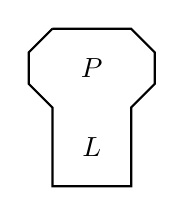
\begin{tikzpicture}
        \draw[thick] (0, 0) -- (1, 0) 
            -- (1.3, -0.3)
            -- (1.3, -0.7)
            -- (1, -1)
            -- (1, -2)
            -- (0, -2)
            -- (0, -1)
            -- (-0.3, -0.7)
            -- (-0.3, -0.3)
            -- (0, 0);
            \node at (0.5, -0.5) {$P$};
            \node at (0.5, -1.5) {$L$};
        \end{tikzpicture}
        \caption{A tombstone diagram for a program $P$ in language $L$.}
    \end{figure}
    
    \item The following figure is used to denote a translator.
    \begin{figure}[H]
        \centering
        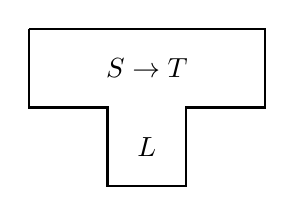
\begin{tikzpicture}
        \draw[thick] (0, 0) -- (3, 0)
            -- (3, -1)
            -- (2, -1)
            -- (2, -2)
            -- (1, -2)
            -- (1, -1)
            -- (0, -1)
            -- (0, 0);
        \node at (1.5, -0.5) {$S \to T$};
        \node at (1.5, -1.5) {$L$};
        \end{tikzpicture}
        \caption{An $S \to T$ translator expressed in the language $L$.}
    \end{figure}
    
    \item The following figure is used to denote an interpreter
    \begin{figure}[H]
        \centering
        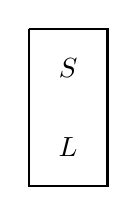
\begin{tikzpicture}
        \draw[thick] (0, 0) -- (1, 0)
            -- (1, -2)
            -- (0, -2)
            -- (0, 0);
        \node at (0.5, -0.5) {$S$};
        \node at (0.5, -1.5) {$L$};
        \end{tikzpicture}
        \caption{An $S$ interpreter in the language $L$.}
    \end{figure}
    
    \item The following figure is used to denote a hardware.
    \begin{figure}[H]
        \centering
        
\begin{tikzpicture}
        \draw[thick] (0, 0) -- (1, 0)
            -- (1, -0.3)
            -- (0.5, -1)
            -- (0, -0.3)
            -- (0, 0);
        \node at (0.5, -0.3) {$M$};
        \end{tikzpicture}
        \caption{A machine $M$ which can only execute $M$'s machine code.}
    \end{figure}
\end{itemize}

We will now look at some concrete examples of tombstone diagrams. 
\begin{itemize}
    \item We can denote the the program \texttt{sort} written in 3 different languages- Java, JVM and x86.
    \begin{figure}[H]
        \centering
        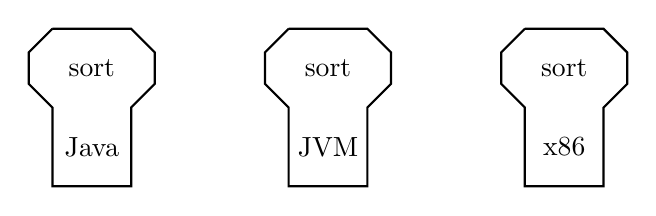
\begin{tikzpicture}
            \draw[thick] (0, 0) -- (1, 0) 
            -- (1.3, -0.3)
            -- (1.3, -0.7)
            -- (1, -1)
            -- (1, -2)
            -- (0, -2)
            -- (0, -1)
            -- (-0.3, -0.7)
            -- (-0.3, -0.3)
            -- (0, 0);
            \node at (0.5, -0.5) {sort};
            \node at (0.5, -1.5) {Java};
            
            \draw[thick] (0+3, 0) -- (1+3, 0) 
            -- (1.3+3, -0.3)
            -- (1.3+3, -0.7)
            -- (1+3, -1)
            -- (1+3, -2)
            -- (0+3, -2)
            -- (0+3, -1)
            -- (-0.3+3, -0.7)
            -- (-0.3+3, -0.3)
            -- (0+3, 0);
            \node at (0.5+3, -0.5) {sort};
            \node at (0.5+3, -1.5) {JVM};
            
            \draw[thick] (0+6, 0) -- (1+6, 0) 
            -- (1.3+6, -0.3)
            -- (1.3+6, -0.7)
            -- (1+6, -1)
            -- (1+6, -2)
            -- (0+6, -2)
            -- (0+6, -1)
            -- (-0.3+6, -0.7)
            -- (-0.3+6, -0.3)
            -- (0+6, 0);
            \node at (0.5+6, -0.5) {sort};
            \node at (0.5+6, -1.5) {x86};
        \end{tikzpicture}
    \end{figure}
    
    \item We can denote the interpreters: a JVM interpreter in C, a JVM interpreter in x86 and a Ruby interpreter in x86.
    \begin{figure}[H]
        \centering
        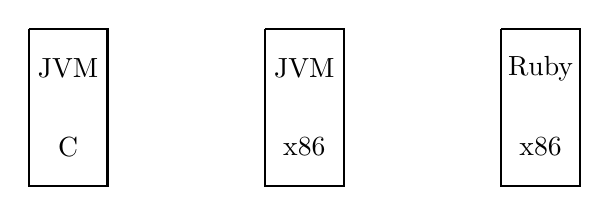
\begin{tikzpicture}
        \draw[thick] (0, 0) -- (1, 0)
            -- (1, -2)
            -- (0, -2)
            -- (0, 0);
        \node at (0.5, -0.5) {JVM};
        \node at (0.5, -1.5) {C};
    
    
        \draw[thick] (0+3, 0) -- (1+3, 0)
            -- (1+3, -2)
            -- (0+3, -2)
            -- (0+3, 0);
        \node at (0.5+3, -0.5) {JVM};
        \node at (0.5+3, -1.5) {x86};
    
    
        \draw[thick] (0+6, 0) -- (1+6, 0)
            -- (1+6, -2)
            -- (0+6, -2)
            -- (0+6, 0);
        \node at (0.5+6, -0.5) {Ruby};
        \node at (0.5+6, -1.5) {x86};
        \end{tikzpicture}
    \end{figure}
    
    \item We can denote the translators: a Java $\to$ JVM compiler in Java, a Java $\to$ C transpiler, an x86as $\to$ x86 assembler in x86, and a JVM $\to$ Java decompiler in C.
    \begin{figure}[H]
        \centering
        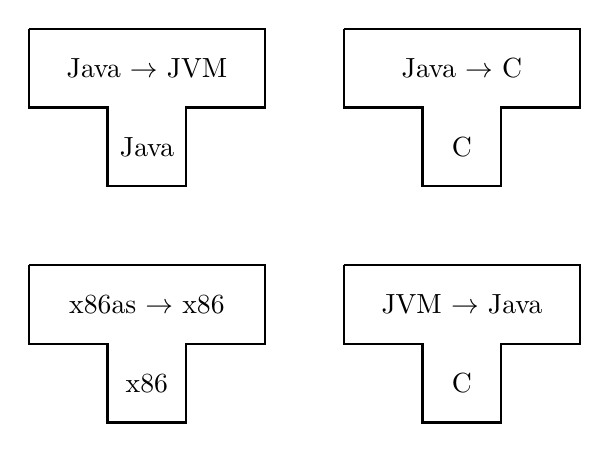
\begin{tikzpicture}
        \draw[thick] (0, 0) -- (3, 0)
            -- (3, -1)
            -- (2, -1)
            -- (2, -2)
            -- (1, -2)
            -- (1, -1)
            -- (0, -1)
            -- (0, 0);
        \node at (1.5, -0.5) {Java $\to$ JVM};
        \node at (1.5, -1.5) {Java};
        
        \draw[thick] (0+4, 0) -- (3+4, 0)
            -- (3+4, -1)
            -- (2+4, -1)
            -- (2+4, -2)
            -- (1+4, -2)
            -- (1+4, -1)
            -- (0+4, -1)
            -- (0+4, 0);
        \node at (1.5+4, -0.5) {Java $\to$ C};
        \node at (1.5+4, -1.5) {C};
        
        \draw[thick] (0, 0-3) -- (3, 0-3)
            -- (3, -1-3)
            -- (2, -1-3)
            -- (2, -2-3)
            -- (1, -2-3)
            -- (1, -1-3)
            -- (0, -1-3)
            -- (0, 0-3);
        \node at (1.5, -0.5-3) {x86as $\to$ x86};
        \node at (1.5, -1.5-3) {x86};
        
        \draw[thick] (0+4, 0-3) -- (3+4, 0-3)
            -- (3+4, -1-3)
            -- (2+4, -1-3)
            -- (2+4, -2-3)
            -- (1+4, -2-3)
            -- (1+4, -1-3)
            -- (0+4, -1-3)
            -- (0+4, 0-3);
        \node at (1.5+4, -0.5-3) {JVM $\to$ Java};
        \node at (1.5+4, -1.5-3) {C};
        \end{tikzpicture}
    \end{figure}
\end{itemize}

We can use tombstone diagrams to run programs. Given a program $P$ expressed in $M$ machine code, we can run $P$ on machine $M$.
\begin{figure}[H]
    \centering
    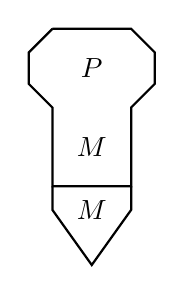
\begin{tikzpicture}
    \draw[thick] (0, 0) -- (1, 0) 
        -- (1.3, -0.3)
        -- (1.3, -0.7)
        -- (1, -1)
        -- (1, -2)
        -- (0, -2)
        -- (0, -1)
        -- (-0.3, -0.7)
        -- (-0.3, -0.3)
        -- (0, 0);
    \node at (0.5, -0.5) {$P$};
    \node at (0.5, -1.5) {$M$};

    \draw[thick] (1, 0-2) -- (1, -0.3-2)
        -- (0.5, -1-2)
        -- (0, -0.3-2)
        -- (0, 0-2);
    \node at (0.5, -0.3-2) {$M$};
    \end{tikzpicture}
    \caption{Running a program $P$ written in $M$.}
\end{figure}
\noindent Note that the two $M$'s must match for the program to run. So, we can run the sort program in x86 and ARM given the right hardware.
\begin{figure}[H]
    \centering
    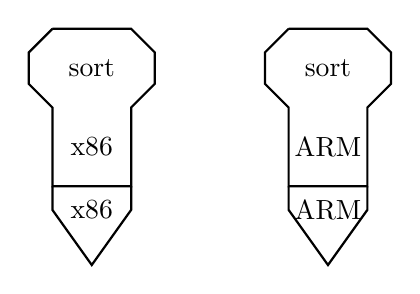
\begin{tikzpicture}
    \draw[thick] (0, 0) -- (1, 0) 
        -- (1.3, -0.3)
        -- (1.3, -0.7)
        -- (1, -1)
        -- (1, -2)
        -- (0, -2)
        -- (0, -1)
        -- (-0.3, -0.7)
        -- (-0.3, -0.3)
        -- (0, 0);
    \node at (0.5, -0.5) {sort};
    \node at (0.5, -1.5) {x86};

    \draw[thick] (1, 0-2) -- (1, -0.3-2)
        -- (0.5, -1-2)
        -- (0, -0.3-2)
        -- (0, 0-2);
    \node at (0.5, -0.3-2) {x86};
    
    \draw[thick] (0+3, 0) -- (1+3, 0) 
        -- (1.3+3, -0.3)
        -- (1.3+3, -0.7)
        -- (1+3, -1)
        -- (1+3, -2)
        -- (0+3, -2)
        -- (0+3, -1)
        -- (-0.3+3, -0.7)
        -- (-0.3+3, -0.3)
        -- (0+3, 0);
    \node at (0.5+3, -0.5) {sort};
    \node at (0.5+3, -1.5) {ARM};

    \draw[thick] (1+3, 0-2) -- (1+3, -0.3-2)
        -- (0.5+3, -1-2)
        -- (0+3, -0.3-2)
        -- (0+3, 0-2);
    \node at (0.5+3, -0.3-2) {ARM};
    \end{tikzpicture}
\end{figure}
\noindent However, the following are not possible since the language of the program doesn't match the hardware.
\begin{figure}[H]
    \centering
    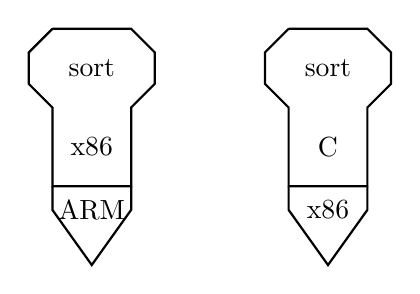
\begin{tikzpicture}
    \draw[thick] (0, 0-4) -- (1, 0-4) 
        -- (1.3, -0.3-4)
        -- (1.3, -0.7-4)
        -- (1, -1-4)
        -- (1, -2-4)
        -- (0, -2-4)
        -- (0, -1-4)
        -- (-0.3, -0.7-4)
        -- (-0.3, -0.3-4)
        -- (0, 0-4);
    \node at (0.5, -0.5-4) {sort};
    \node at (0.5, -1.5-4) {x86};

    \draw[thick] (1, 0-2-4) -- (1, -0.3-2-4)
        -- (0.5, -1-2-4)
        -- (0, -0.3-2-4)
        -- (0, 0-2-4);
    \node at (0.5, -0.3-2-4) {ARM};
    
    \draw[thick] (0+3, 0-4) -- (1+3, 0-4) 
        -- (1.3+3, -0.3-4)
        -- (1.3+3, -0.7-4)
        -- (1+3, -1-4)
        -- (1+3, -2-4)
        -- (0+3, -2-4)
        -- (0+3, -1-4)
        -- (-0.3+3, -0.7-4)
        -- (-0.3+3, -0.3-4)
        -- (0+3, 0-4);
    \node at (0.5+3, -0.5-4) {sort};
    \node at (0.5+3, -1.5-4) {C};

    \draw[thick] (1+3, 0-2-4) -- (1+3, -0.3-2-4)
        -- (0.5+3, -1-2-4)
        -- (0+3, -0.3-2-4)
        -- (0+3, 0-2-4);
    \node at (0.5+3, -0.3-2-4) {x86};
    \end{tikzpicture}
\end{figure}

We can also show the translation of a program via tombstone diagrams. Given an $S \to T$ translator, expressed in $M$ machine code, and a program $P$ expressed in language $S$, we can translate $P$ to language $T$.
\begin{figure}[H]
    \centering
    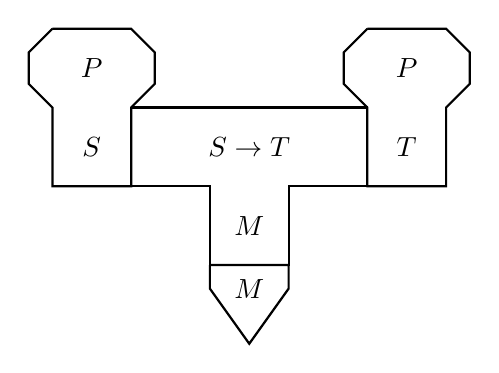
\begin{tikzpicture}
    \draw[thick] (0, 0) -- (1, 0) 
        -- (1.3, -0.3)
        -- (1.3, -0.7)
        -- (1, -1)
        -- (1, -2)
        -- (0, -2)
        -- (0, -1)
        -- (-0.3, -0.7)
        -- (-0.3, -0.3)
        -- (0, 0);
        \node at (0.5, -0.5) {$P$};
        \node at (0.5, -1.5) {$S$};
        
      \draw[thick] (0+1, 0-1) -- (3+1, 0-1)
        -- (3+1, -1-1)
        -- (2+1, -1-1)
        -- (2+1, -2-1)
        -- (1+1, -2-1)
        -- (1+1, -1-1)
        -- (0+1, -1-1)
        -- (0+1, 0-1);
    \node at (1.5+1, -0.5-1) {$S \to T$};
    \node at (1.5+1, -1.5-1) {$M$};

    \draw[thick] (0+4, 0) -- (1+4, 0) 
        -- (1.3+4, -0.3)
        -- (1.3+4, -0.7)
        -- (1+4, -1)
        -- (1+4, -2)
        -- (0+4, -2)
        -- (0+4, -1)
        -- (-0.3+4, -0.7)
        -- (-0.3+4, -0.3)
        -- (0+4, 0);
        \node at (0.5+4, -0.5) {$P$};
        \node at (0.5+4, -1.5) {$T$};

    \draw[thick] (0+2, 0-3) -- (1+2, 0-3)
        -- (1+2, -0.3-3)
        -- (0.5+2, -1-3)
        -- (0+2, -0.3-3)
        -- (0+2, 0-3);
    \node at (0.5+2, -0.3-3) {$M$};
    \end{tikzpicture}
\end{figure}
\noindent Note that the PLs must match the source and the target languages of the translator. Also, the language of the translator must match the language of the hardware. An example of this is given below- compiling the sort program from C to x86.
\begin{figure}[H]
    \centering
    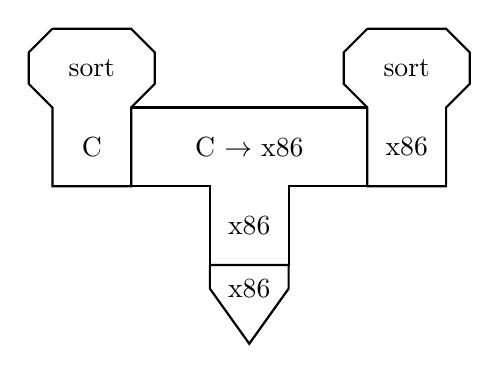
\begin{tikzpicture}
    \draw[thick] (0, 0) -- (1, 0) 
        -- (1.3, -0.3)
        -- (1.3, -0.7)
        -- (1, -1)
        -- (1, -2)
        -- (0, -2)
        -- (0, -1)
        -- (-0.3, -0.7)
        -- (-0.3, -0.3)
        -- (0, 0);
        \node at (0.5, -0.5) {sort};
        \node at (0.5, -1.5) {C};
        
      \draw[thick] (0+1, 0-1) -- (3+1, 0-1)
        -- (3+1, -1-1)
        -- (2+1, -1-1)
        -- (2+1, -2-1)
        -- (1+1, -2-1)
        -- (1+1, -1-1)
        -- (0+1, -1-1)
        -- (0+1, 0-1);
    \node at (1.5+1, -0.5-1) {C $\to$ x86};
    \node at (1.5+1, -1.5-1) {x86};

    \draw[thick] (0+4, 0) -- (1+4, 0) 
        -- (1.3+4, -0.3)
        -- (1.3+4, -0.7)
        -- (1+4, -1)
        -- (1+4, -2)
        -- (0+4, -2)
        -- (0+4, -1)
        -- (-0.3+4, -0.7)
        -- (-0.3+4, -0.3)
        -- (0+4, 0);
        \node at (0.5+4, -0.5) {sort};
        \node at (0.5+4, -1.5) {x86};

    \draw[thick] (0+2, 0-3) -- (1+2, 0-3)
        -- (1+2, -0.3-3)
        -- (0.5+2, -1-3)
        -- (0+2, -0.3-3)
        -- (0+2, 0-3);
    \node at (0.5+2, -0.3-3) {x86};
    \end{tikzpicture}
\end{figure}
\noindent This represents the compilation of the program. We can later run the object program on an x86, which is depicted by the tombstone diagram below.
\begin{figure}[H]
    \centering
    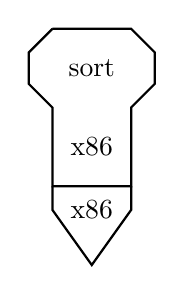
\begin{tikzpicture}
    \draw[thick] (0+3, 0-4) -- (1+3, 0-4) 
        -- (1.3+3, -0.3-4)
        -- (1.3+3, -0.7-4)
        -- (1+3, -1-4)
        -- (1+3, -2-4)
        -- (0+3, -2-4)
        -- (0+3, -1-4)
        -- (-0.3+3, -0.7-4)
        -- (-0.3+3, -0.3-4)
        -- (0+3, 0-4);
    \node at (0.5+3, -0.5-4) {sort};
    \node at (0.5+3, -1.5-4) {x86};

    \draw[thick] (1+3, 0-2-4) -- (1+3, -0.3-2-4)
        -- (0.5+3, -1-2-4)
        -- (0+3, -0.3-2-4)
        -- (0+3, 0-2-4);
    \node at (0.5+3, -0.3-2-4) {x86};
    \end{tikzpicture}
\end{figure}
\noindent This represents the runtime of the program.

We could break the compilation into 2 steps. For example, we can have a C $\to$ x86as compiler, and an x86 assembler. Then, we can use them to compile a program in C into x86 machine code, in 2 stages.
\begin{figure}[H]
    \centering
    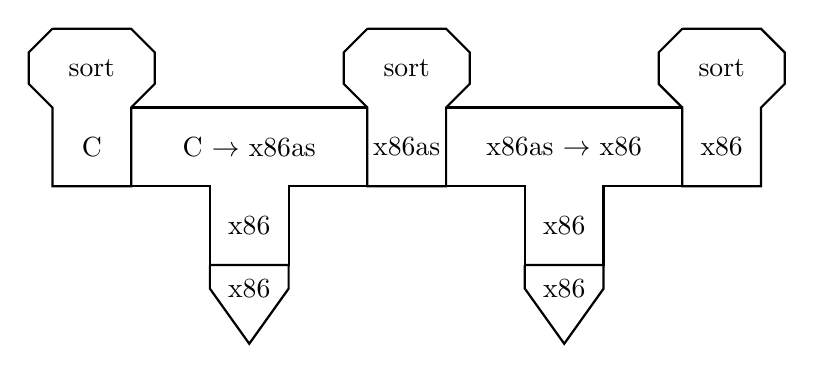
\begin{tikzpicture}
    \draw[thick] (0, 0) -- (1, 0) 
        -- (1.3, -0.3)
        -- (1.3, -0.7)
        -- (1, -1)
        -- (1, -2)
        -- (0, -2)
        -- (0, -1)
        -- (-0.3, -0.7)
        -- (-0.3, -0.3)
        -- (0, 0);
        \node at (0.5, -0.5) {sort};
        \node at (0.5, -1.5) {C};
        
      \draw[thick] (0+1, 0-1) -- (3+1, 0-1)
        -- (3+1, -1-1)
        -- (2+1, -1-1)
        -- (2+1, -2-1)
        -- (1+1, -2-1)
        -- (1+1, -1-1)
        -- (0+1, -1-1)
        -- (0+1, 0-1);
    \node at (1.5+1, -0.5-1) {C $\to$ x86as};
    \node at (1.5+1, -1.5-1) {x86};

    \draw[thick] (0+4, 0) -- (1+4, 0) 
        -- (1.3+4, -0.3)
        -- (1.3+4, -0.7)
        -- (1+4, -1)
        -- (1+4, -2)
        -- (0+4, -2)
        -- (0+4, -1)
        -- (-0.3+4, -0.7)
        -- (-0.3+4, -0.3)
        -- (0+4, 0);
        \node at (0.5+4, -0.5) {sort};
        \node at (0.5+4, -1.5) {x86as};

    \draw[thick] (0+2, 0-3) -- (1+2, 0-3)
        -- (1+2, -0.3-3)
        -- (0.5+2, -1-3)
        -- (0+2, -0.3-3)
        -- (0+2, 0-3);
    \node at (0.5+2, -0.3-3) {x86};
        
     \draw[thick] (0+5, 0-1) -- (3+5, 0-1)
        -- (3+5, -1-1)
        -- (2+5, -1-1)
        -- (2+5, -2-1)
        -- (1+5, -2-1)
        -- (1+5, -1-1)
        -- (0+5, -1-1)
        -- (0+5, 0-1);
    \node at (1.5+5, -0.5-1) {x86as $\to$ x86};
    \node at (1.5+5, -1.5-1) {x86};

    \draw[thick] (0+8, 0) -- (1+8, 0) 
        -- (1.3+8, -0.3)
        -- (1.3+8, -0.7)
        -- (1+8, -1)
        -- (1+8, -2)
        -- (0+8, -2)
        -- (0+8, -1)
        -- (-0.3+8, -0.7)
        -- (-0.3+8, -0.3)
        -- (0+8, 0);
        \node at (0.5+8, -0.5) {sort};
        \node at (0.5+8, -1.5) {x86};

    \draw[thick] (0+6, 0-3) -- (1+6, 0-3)
        -- (1+6, -0.3-3)
        -- (0.5+6, -1-3)
        -- (0+6, -0.3-3)
        -- (0+6, 0-3);
    \node at (0.5+6, -0.3-3) {x86};
    \end{tikzpicture}
\end{figure}

We can compile a compiler. Given a C $\to$ x86 compiler, we can use it to compile any C program into x86 machine code. In particular, we can compile a compiler expressed in C, e.g. compiling a Java $\to$ JVM compiler written in C to a Java $\to$ JVM compiler in x86.
\begin{figure}[H]
    \centering
    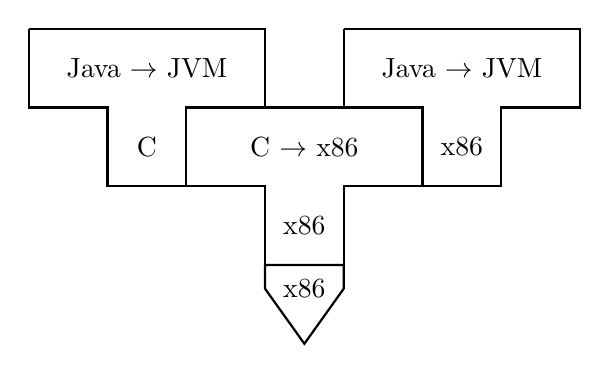
\begin{tikzpicture}
    \draw[thick] (0-1, 0) -- (3-1, 0)
        -- (3-1, -1)
        -- (2-1, -1)
        -- (2-1, -2)
        -- (1-1, -2)
        -- (1-1, -1)
        -- (0-1, -1)
        -- (0-1, 0);
    \node at (1.5-1, -0.5) {Java $\to$ JVM};
    \node at (1.5-1, -1.5) {C};
        
      \draw[thick] (0+1, 0-1) -- (3+1, 0-1)
        -- (3+1, -1-1)
        -- (2+1, -1-1)
        -- (2+1, -2-1)
        -- (1+1, -2-1)
        -- (1+1, -1-1)
        -- (0+1, -1-1)
        -- (0+1, 0-1);
    \node at (1.5+1, -0.5-1) {C $\to$ x86};
    \node at (1.5+1, -1.5-1) {x86};

    \draw[thick] (0+3, 0) -- (3+3, 0)
        -- (3+3, -1)
        -- (2+3, -1)
        -- (2+3, -2)
        -- (1+3, -2)
        -- (1+3, -1)
        -- (0+3, -1)
        -- (0+3, 0);
    \node at (1.5+3, -0.5) {Java $\to$ JVM};
    \node at (1.5+3, -1.5) {x86};

    \draw[thick] (0+2, 0-3) -- (1+2, 0-3)
        -- (1+2, -0.3-3)
        -- (0.5+2, -1-3)
        -- (0+2, -0.3-3)
        -- (0+2, 0-3);
    \node at (0.5+2, -0.3-3) {x86};
    \end{tikzpicture}
\end{figure}
\noindent For this to be possible, we require the relevant languages to match. So, the following is possible.
\begin{figure}[H]
    \centering
    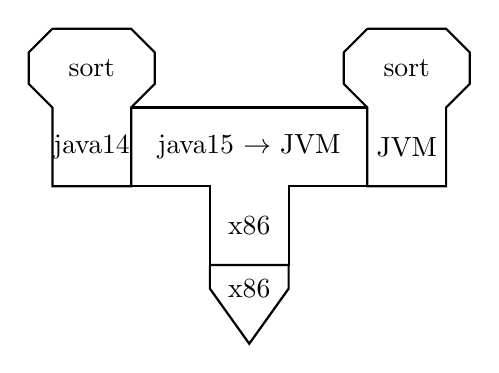
\begin{tikzpicture}
    \draw[thick] (0, 0) -- (1, 0) 
        -- (1.3, -0.3)
        -- (1.3, -0.7)
        -- (1, -1)
        -- (1, -2)
        -- (0, -2)
        -- (0, -1)
        -- (-0.3, -0.7)
        -- (-0.3, -0.3)
        -- (0, 0);
        \node at (0.5, -0.5) {sort};
        \node at (0.5, -1.5) {java14};
        
      \draw[thick] (0+1, 0-1) -- (3+1, 0-1)
        -- (3+1, -1-1)
        -- (2+1, -1-1)
        -- (2+1, -2-1)
        -- (1+1, -2-1)
        -- (1+1, -1-1)
        -- (0+1, -1-1)
        -- (0+1, 0-1);
    \node at (1.5+1, -0.5-1) {java15 $\to$ JVM};
    \node at (1.5+1, -1.5-1) {x86};

    \draw[thick] (0+4, 0) -- (1+4, 0) 
        -- (1.3+4, -0.3)
        -- (1.3+4, -0.7)
        -- (1+4, -1)
        -- (1+4, -2)
        -- (0+4, -2)
        -- (0+4, -1)
        -- (-0.3+4, -0.7)
        -- (-0.3+4, -0.3)
        -- (0+4, 0);
        \node at (0.5+4, -0.5) {sort};
        \node at (0.5+4, -1.5) {JVM};

    \draw[thick] (0+2, 0-3) -- (1+2, 0-3)
        -- (1+2, -0.3-3)
        -- (0.5+2, -1-3)
        -- (0+2, -0.3-3)
        -- (0+2, 0-3);
    \node at (0.5+2, -0.3-3) {x86};
    \end{tikzpicture}
\end{figure}
\noindent This is because Java14 is a subset of Java15. However, we cannot run a C $\to$ x86 compiler in an ARM hardware.
\begin{figure}[H]
    \centering
    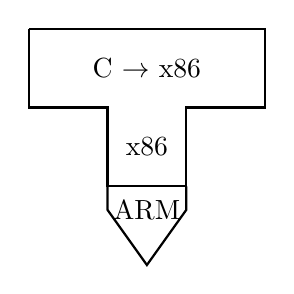
\begin{tikzpicture}
    \draw[thick] (0+1, 0-1) -- (3+1, 0-1)
        -- (3+1, -1-1)
        -- (2+1, -1-1)
        -- (2+1, -2-1)
        -- (1+1, -2-1)
        -- (1+1, -1-1)
        -- (0+1, -1-1)
        -- (0+1, 0-1);
    \node at (1.5+1, -0.5-1) {C $\to$ x86};
    \node at (1.5+1, -1.5-1) {x86};

    \draw[thick] (1+2, 0-3) -- (1+2, -0.3-3)
        -- (0.5+2, -1-3)
        -- (0+2, -0.3-3)
        -- (0+2, 0-3);
    \node at (0.5+2, -0.3-3) {ARM};
    \end{tikzpicture}
\end{figure}
\noindent Similarly, we cannot compile a Java program using a C $\to$ x86 compiler.
\begin{figure}[H]
    \centering
    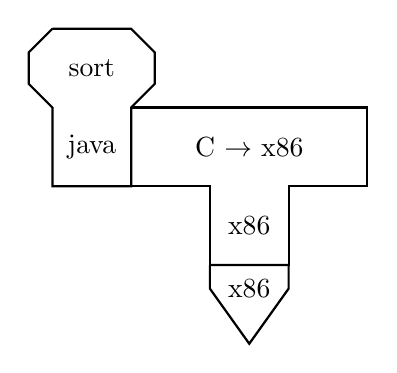
\begin{tikzpicture}
    \draw[thick] (0, 0) -- (1, 0) 
        -- (1.3, -0.3)
        -- (1.3, -0.7)
        -- (1, -1)
        -- (1, -2)
        -- (0, -2)
        -- (0, -1)
        -- (-0.3, -0.7)
        -- (-0.3, -0.3)
        -- (0, 0);
        \node at (0.5, -0.5) {sort};
        \node at (0.5, -1.5) {java};
        
      \draw[thick] (0+1, 0-1) -- (3+1, 0-1)
        -- (3+1, -1-1)
        -- (2+1, -1-1)
        -- (2+1, -2-1)
        -- (1+1, -2-1)
        -- (1+1, -1-1)
        -- (0+1, -1-1)
        -- (0+1, 0-1);
    \node at (1.5+1, -0.5-1) {C $\to$ x86};
    \node at (1.5+1, -1.5-1) {x86};

    \draw[thick] (0+2, 0-3) -- (1+2, 0-3)
        -- (1+2, -0.3-3)
        -- (0.5+2, -1-3)
        -- (0+2, -0.3-3)
        -- (0+2, 0-3);
    \node at (0.5+2, -0.3-3) {x86};
    \end{tikzpicture}
\end{figure}

Now, we will consider representing interpretation via tombstone diagrams. Given an $S$ interpreter expressed in $M$ machine code and a program $P$ expressed in language $S$, we can interpret $P$. This is denoted as follows.
\begin{figure}[H]
    \centering
    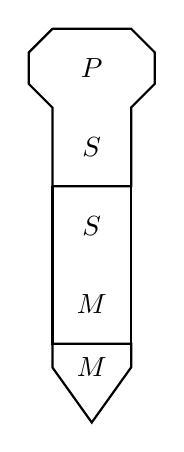
\begin{tikzpicture}
    \draw[thick] (0, 0) -- (1, 0) 
        -- (1.3, -0.3)
        -- (1.3, -0.7)
        -- (1, -1)
        -- (1, -2)
        -- (0, -2)
        -- (0, -1)
        -- (-0.3, -0.7)
        -- (-0.3, -0.3)
        -- (0, 0);
    \node at (0.5, -0.5) {$P$};
    \node at (0.5, -1.5) {$S$};
    
    \draw[thick] (1, -3) -- (1, -2)
        -- (1, -4) 
        -- (0, -4)
        -- (0, -2);
    \node at (0.5, -2.5) {$S$};
    \node at (0.5, -3.5) {$M$};
    
    \draw[thick] (0, 0-4) -- (1, 0-4)
        -- (1, -0.3-4)
        -- (0.5, -1-4)
        -- (0, -0.3-4)
        -- (0, 0-4);
    \node at (0.5, -0.3-4) {$M$};
    \end{tikzpicture}
\end{figure}
\noindent The language in which the program is written (i.e. $S$) must match the language that is being interpreted. Moreover, the language in which the interpreter is written (i.e. $M$) must match the language of the hardware. So, it is possible to interpret a sort program in Ruby with a Ruby interpreter, but not a sort program in C.
\begin{figure}[H]
    \centering
    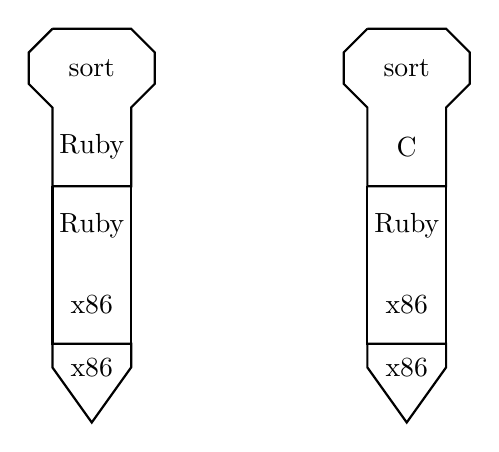
\begin{tikzpicture}
    \draw[thick] (0, 0) -- (1, 0) 
        -- (1.3, -0.3)
        -- (1.3, -0.7)
        -- (1, -1)
        -- (1, -2)
        -- (0, -2)
        -- (0, -1)
        -- (-0.3, -0.7)
        -- (-0.3, -0.3)
        -- (0, 0);
    \node at (0.5, -0.5) {sort};
    \node at (0.5, -1.5) {Ruby};
    
    \draw[thick] (1, -3) -- (1, -2)
        -- (1, -4) 
        -- (0, -4)
        -- (0, -2);
    \node at (0.5, -2.5) {Ruby};
    \node at (0.5, -3.5) {x86};
    
    \draw[thick] (0, 0-4) -- (1, 0-4)
        -- (1, -0.3-4)
        -- (0.5, -1-4)
        -- (0, -0.3-4)
        -- (0, 0-4);
    \node at (0.5, -0.3-4) {x86};

    \draw[thick] (0+4, 0) -- (1+4, 0) 
        -- (1.3+4, -0.3)
        -- (1.3+4, -0.7)
        -- (1+4, -1)
        -- (1+4, -2)
        -- (0+4, -2)
        -- (0+4, -1)
        -- (-0.3+4, -0.7)
        -- (-0.3+4, -0.3)
        -- (0+4, 0);
    \node at (0.5+4, -0.5) {sort};
    \node at (0.5+4, -1.5) {C};
    
    \draw[thick] (1+4, -3) -- (1+4, -2)
        -- (1+4, -4) 
        -- (0+4, -4)
        -- (0+4, -2);
    \node at (0.5+4, -2.5) {Ruby};
    \node at (0.5+4, -3.5) {x86};
    
    \draw[thick] (0+4, 0-4) -- (1+4, 0-4)
        -- (1+4, -0.3-4)
        -- (0.5+4, -1-4)
        -- (0+4, -0.3-4)
        -- (0+4, 0-4);
    \node at (0.5+4, -0.3-4) {x86};
    \end{tikzpicture}
\end{figure}

\subsection{Virtual machines}
A real machine is one whose machine code is executed by hardware. A virtual machine (or an abstract machine) is one whose machine code is executed by an interpreter. We can use tombstone diagrams to denote virtual machines. For example, assume that we designed the architecture and instruction set of a new machine called MVM. Building a hardware prototype would be expensive, and even more to modify.

We can first write an interpreter for MVM machine code (an emulator) expressed in C, for example. This is given below.
\begin{figure}[H]
    \centering
    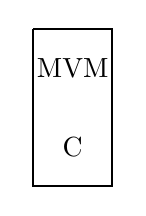
\begin{tikzpicture}
    \draw[thick] (0, 0) -- (1, 0)
        -- (1, -2)
        -- (0, -2)
        -- (0, 0);
    \node at (0.5, -0.5) {MVM};
    \node at (0.5, -1.5) {C};
    \end{tikzpicture}
\end{figure}
\noindent We can then compile it on a real machine, e.g. x86.
\begin{figure}[H]
    \centering
    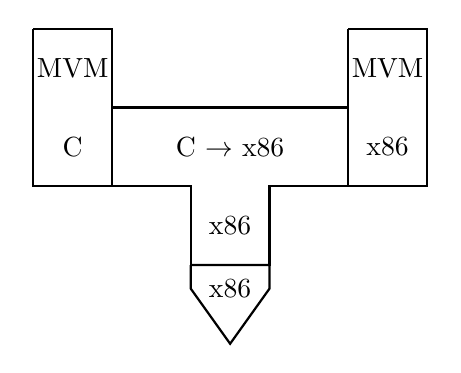
\begin{tikzpicture}
    \draw[thick] (0, 0) -- (1, 0)
        -- (1, -2)
        -- (0, -2)
        -- (0, 0);
    \node at (0.5, -0.5) {MVM};
    \node at (0.5, -1.5) {C};
        
      \draw[thick] (0+1, 0-1) -- (3+1, 0-1)
        -- (3+1, -1-1)
        -- (2+1, -1-1)
        -- (2+1, -2-1)
        -- (1+1, -2-1)
        -- (1+1, -1-1)
        -- (0+1, -1-1)
        -- (0+1, 0-1);
    \node at (1.5+1, -0.5-1) {C $\to$ x86};
    \node at (1.5+1, -1.5-1) {x86};

    \draw[thick] (0+4, 0) -- (1+4, 0)
        -- (1+4, -2)
        -- (0+4, -2)
        -- (0+4, 0);
    \node at (0.5+4, -0.5) {MVM};
    \node at (0.5+4, -1.5) {x86};

    \draw[thick] (0+2, 0-3) -- (1+2, 0-3)
        -- (1+2, -0.3-3)
        -- (0.5+2, -1-3)
        -- (0+2, -0.3-3)
        -- (0+2, 0-3);
    \node at (0.5+2, -0.3-3) {x86};
    \end{tikzpicture}
\end{figure}
\noindent Now, we can use the emulator to execute programs $P$ expressed in MVM machine code.
\begin{figure}[H]
    \centering
    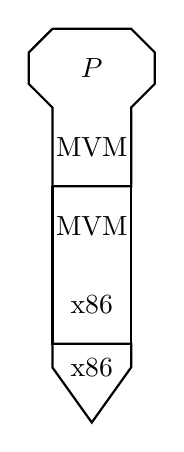
\begin{tikzpicture}
    \draw[thick] (0, 0) -- (1, 0) 
        -- (1.3, -0.3)
        -- (1.3, -0.7)
        -- (1, -1)
        -- (1, -2)
        -- (0, -2)
        -- (0, -1)
        -- (-0.3, -0.7)
        -- (-0.3, -0.3)
        -- (0, 0);
    \node at (0.5, -0.5) {$P$};
    \node at (0.5, -1.5) {MVM};
    
    \draw[thick] (1, -3) -- (1, -2)
        -- (1, -4) 
        -- (0, -4)
        -- (0, -2);
    \node at (0.5, -2.5) {MVM};
    \node at (0.5, -3.5) {x86};
    
    \draw[thick] (0, 0-4) -- (1, 0-4)
        -- (1, -0.3-4)
        -- (0.5, -1-4)
        -- (0, -0.3-4)
        -- (0, 0-4);
    \node at (0.5, -0.3-4) {x86};
    \end{tikzpicture}
\end{figure}
\noindent The bottom two layers are called the MVM virtual machine. This has the same effect as the MVM real machine, given by the following.
\begin{figure}[H]
    \centering
    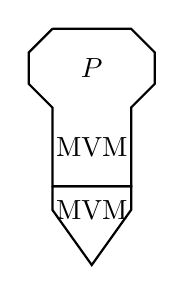
\begin{tikzpicture}
    \draw[thick] (0+4, 0) -- (1+4, 0) 
        -- (1.3+4, -0.3)
        -- (1.3+4, -0.7)
        -- (1+4, -1)
        -- (1+4, -2)
        -- (0+4, -2)
        -- (0+4, -1)
        -- (-0.3+4, -0.7)
        -- (-0.3+4, -0.3)
        -- (0+4, 0);
    \node at (0.5+4, -0.5) {$P$};
    \node at (0.5+4, -1.5) {MVM};
    
    \draw[thick] (0+4, 0-2) -- (1+4, 0-2)
        -- (1+4, -0.3-2)
        -- (0.5+4, -1-2)
        -- (0+4, -0.3-2)
        -- (0+4, 0-2);
    \node at (0.5+4, -0.3-2) {MVM};
    \end{tikzpicture}
\end{figure}
\noindent However, using the MVM real machine would be much faster.

\subsection{Interpretive Compilers}
A compiler takes quite a long time to translate the source program to native machine code, but the subsequent execution is fast. On the other hand, an interpreter starts executing the source program immediately, but the execution is slow. We can combine the two and get an interpretive compiler. It translates the source program into virtual machine (VM) code which is subsequently interpreted.

An interpretive compiler combines fast translation with moderately fast execution, provided that:
\begin{itemize}
    \item the VM code is intermediate-level (lower-level than the source code but higher-level than native machine code);
    \item translation from the source language to VM code is easy and fast;
    \item the VM instructions have simpler formats (so can be analysed quickly by an interpreter).
\end{itemize}

For example, JDK (Java development kit) provides an interpretive compiler for Java. This is based on the JVM (Java virtual machine) that was designed to run Java programs. JVM provides powerful instructions that implement object creation, method calls, array indexing, etc. However, the instructions (called `bytecodes') are similar in format to native machine code, i.e. opcode + operand.

JDK comprises a Java $\to$ JVM compiler and a JVM interpreter. Once JDK has been installed on a real machine, we have the following components:
\begin{figure}[H]
    \centering
    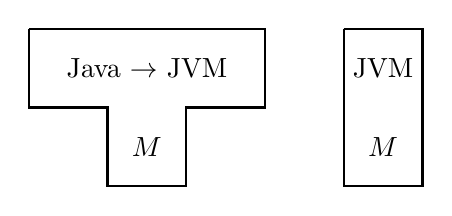
\begin{tikzpicture}
    \draw[thick] (0, 0) -- (3, 0)
        -- (3, -1)
        -- (2, -1)
        -- (2, -2)
        -- (1, -2)
        -- (1, -1)
        -- (0, -1)
        -- (0, 0);
    \node at (1.5, -0.5) {Java $\to$ JVM};
    \node at (1.5, -1.5) {$M$};

    \draw[thick] (0+4, 0) -- (1+4, 0)
        -- (1+4, -2)
        -- (0+4, -2)
        -- (0+4, 0);
    \node at (0.5+4, -0.5) {JVM};
    \node at (0.5+4, -1.5) {$M$};
    \end{tikzpicture}
\end{figure}
\noindent Using these, we can translate Java source program $P$ into JVM code.
\begin{figure}[H]
    \centering
    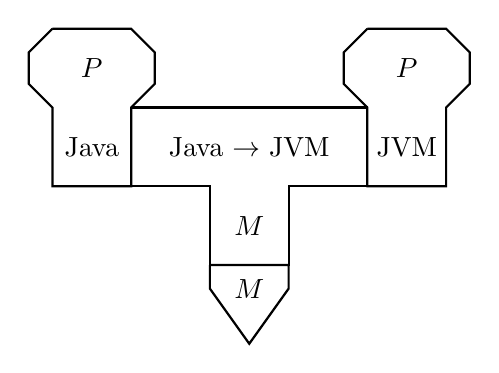
\begin{tikzpicture}
    \draw[thick] (0, 0) -- (1, 0) 
        -- (1.3, -0.3)
        -- (1.3, -0.7)
        -- (1, -1)
        -- (1, -2)
        -- (0, -2)
        -- (0, -1)
        -- (-0.3, -0.7)
        -- (-0.3, -0.3)
        -- (0, 0);
        \node at (0.5, -0.5) {$P$};
        \node at (0.5, -1.5) {Java};
        
      \draw[thick] (0+1, 0-1) -- (3+1, 0-1)
        -- (3+1, -1-1)
        -- (2+1, -1-1)
        -- (2+1, -2-1)
        -- (1+1, -2-1)
        -- (1+1, -1-1)
        -- (0+1, -1-1)
        -- (0+1, 0-1);
    \node at (1.5+1, -0.5-1) {Java $\to$ JVM};
    \node at (1.5+1, -1.5-1) {$M$};

    \draw[thick] (0+4, 0) -- (1+4, 0) 
        -- (1.3+4, -0.3)
        -- (1.3+4, -0.7)
        -- (1+4, -1)
        -- (1+4, -2)
        -- (0+4, -2)
        -- (0+4, -1)
        -- (-0.3+4, -0.7)
        -- (-0.3+4, -0.3)
        -- (0+4, 0);
        \node at (0.5+4, -0.5) {$P$};
        \node at (0.5+4, -1.5) {JVM};

    \draw[thick] (0+2, 0-3) -- (1+2, 0-3)
        -- (1+2, -0.3-3)
        -- (0.5+2, -1-3)
        -- (0+2, -0.3-3)
        -- (0+2, 0-3);
    \node at (0.5+2, -0.3-3) {$M$};
    \end{tikzpicture}
\end{figure}
\noindent Later, the object program is interpreted.
\begin{figure}[H]
    \centering
    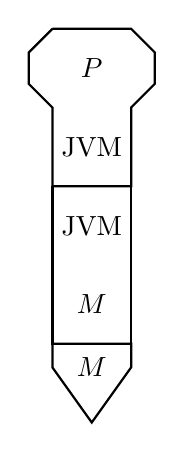
\begin{tikzpicture}
    \draw[thick] (0, 0) -- (1, 0) 
        -- (1.3, -0.3)
        -- (1.3, -0.7)
        -- (1, -1)
        -- (1, -2)
        -- (0, -2)
        -- (0, -1)
        -- (-0.3, -0.7)
        -- (-0.3, -0.3)
        -- (0, 0);
    \node at (0.5, -0.5) {$P$};
    \node at (0.5, -1.5) {JVM};
    
    \draw[thick] (1, -3) -- (1, -2)
        -- (1, -4) 
        -- (0, -4)
        -- (0, -2);
    \node at (0.5, -2.5) {JVM};
    \node at (0.5, -3.5) {$M$};
    
    \draw[thick] (0, 0-4) -- (1, 0-4)
        -- (1, -0.3-4)
        -- (0.5, -1-4)
        -- (0, -0.3-4)
        -- (0, 0-4);
    \node at (0.5, -0.3-4) {$M$};
    \end{tikzpicture}
\end{figure}
\noindent The bottom two tiles are called the Java Virtual Machine.

A just-in-time (JIT) compiler translates virtual machine code to native machine code just prior to execution. More usually, a Java JIT compiler translates JVM code selectively. The interpreter and the JIT compiler work together. The interpreter is instrumented to count method calls. When the interpreter discovers that a method is `hot' (i.e. it is called frequently), it tells the JIT compiler to translate the particular method into native code.

A program is portable if it can be made to run on different machines with minimal change. So, a program $P$ written in Java is portable, but the same program in x86 is not. A compiler that generates native machine code is unportable- if it must be changed to target a different machine, its code generator must be replaced. However, a compiler that generates suitable virtual machine code can be portable.

So, a portable compiler kit for Java is composed of the following tiles:
\begin{figure}[H]
    \centering
    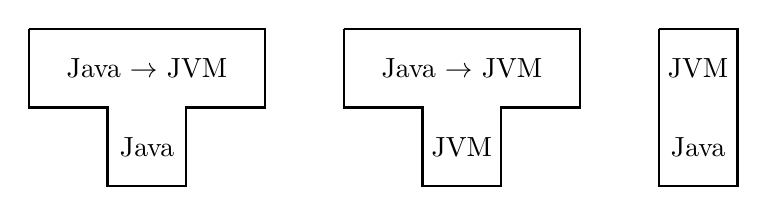
\begin{tikzpicture}
    \draw[thick] (0, 0) -- (3, 0)
        -- (3, -1)
        -- (2, -1)
        -- (2, -2)
        -- (1, -2)
        -- (1, -1)
        -- (0, -1)
        -- (0, 0);
    \node at (1.5, -0.5) {Java $\to$ JVM};
    \node at (1.5, -1.5) {Java};
    
    \draw[thick] (0+4, 0) -- (3+4, 0)
        -- (3+4, -1)
        -- (2+4, -1)
        -- (2+4, -2)
        -- (1+4, -2)
        -- (1+4, -1)
        -- (0+4, -1)
        -- (0+4, 0);
    \node at (1.5+4, -0.5) {Java $\to$ JVM};
    \node at (1.5+4, -1.5) {JVM};

    \draw[thick] (0+8, 0) -- (1+8, 0)
        -- (1+8, -2)
        -- (0+8, -2)
        -- (0+8, 0);
    \node at (0.5+8, -0.5) {JVM};
    \node at (0.5+8, -1.5) {Java};
    \end{tikzpicture}
\end{figure}
\noindent We can install this kit on machine $M$. But, we cannot run the JVM interpreter until we have a running Java compiler. Similarly, we cannot run the Java compiler until we have a running JVM interpreter.

To progress, we first rewrite the JVM interpreter, e.g. in C.
\begin{figure}[H]
    \centering
    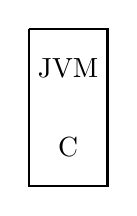
\begin{tikzpicture}
    \draw[thick] (0+8, 0) -- (1+8, 0)
        -- (1+8, -2)
        -- (0+8, -2)
        -- (0+8, 0);
    \node at (0.5+8, -0.5) {JVM};
    \node at (0.5+8, -1.5) {C};
    \end{tikzpicture}
\end{figure}
\noindent Then, we compile the JVM interpreter on $M$.
\begin{figure}[H]
    \centering
    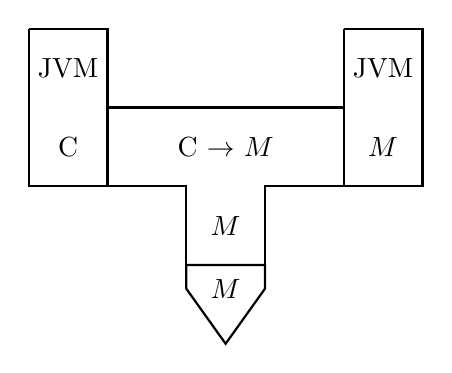
\begin{tikzpicture}
    \draw[thick] (0, 0) -- (1, 0)
        -- (1, -2)
        -- (0, -2)
        -- (0, 0);
    \node at (0.5, -0.5) {JVM};
    \node at (0.5, -1.5) {C};
        
      \draw[thick] (0+1, 0-1) -- (3+1, 0-1)
        -- (3+1, -1-1)
        -- (2+1, -1-1)
        -- (2+1, -2-1)
        -- (1+1, -2-1)
        -- (1+1, -1-1)
        -- (0+1, -1-1)
        -- (0+1, 0-1);
    \node at (1.5+1, -0.5-1) {C $\to$ $M$};
    \node at (1.5+1, -1.5-1) {$M$};

    \draw[thick] (0+4, 0) -- (1+4, 0)
        -- (1+4, -2)
        -- (0+4, -2)
        -- (0+4, 0);
    \node at (0.5+4, -0.5) {JVM};
    \node at (0.5+4, -1.5) {$M$};

    \draw[thick] (0+2, 0-3) -- (1+2, 0-3)
        -- (1+2, -0.3-3)
        -- (0.5+2, -1-3)
        -- (0+2, -0.3-3)
        -- (0+2, 0-3);
    \node at (0.5+2, -0.3-3) {$M$};
    \end{tikzpicture}
\end{figure}
\noindent Now, we have an interpretive compiler. But, the compiler itself must be interpreted in this case.
\begin{figure}[H]
    \centering
    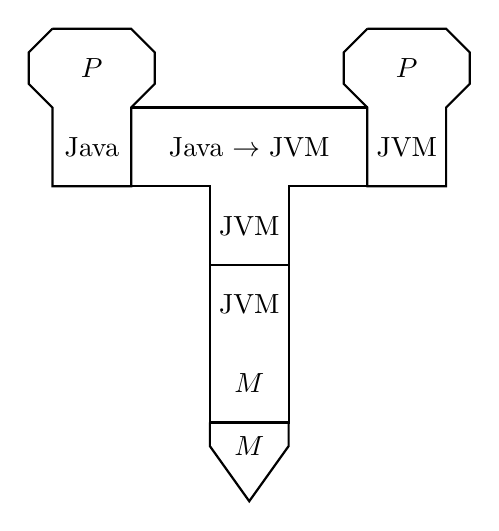
\begin{tikzpicture}
    \draw[thick] (0, 0) -- (1, 0) 
        -- (1.3, -0.3)
        -- (1.3, -0.7)
        -- (1, -1)
        -- (1, -2)
        -- (0, -2)
        -- (0, -1)
        -- (-0.3, -0.7)
        -- (-0.3, -0.3)
        -- (0, 0);
        \node at (0.5, -0.5) {$P$};
        \node at (0.5, -1.5) {Java};
        
      \draw[thick] (0+1, 0-1) -- (3+1, 0-1)
        -- (3+1, -1-1)
        -- (2+1, -1-1)
        -- (2+1, -2-1)
        -- (1+1, -2-1)
        -- (1+1, -1-1)
        -- (0+1, -1-1)
        -- (0+1, 0-1);
    \node at (1.5+1, -0.5-1) {Java $\to$ JVM};
    \node at (1.5+1, -1.5-1) {JVM};

    \draw[thick] (0+4, 0) -- (1+4, 0) 
        -- (1.3+4, -0.3)
        -- (1.3+4, -0.7)
        -- (1+4, -1)
        -- (1+4, -2)
        -- (0+4, -2)
        -- (0+4, -1)
        -- (-0.3+4, -0.7)
        -- (-0.3+4, -0.3)
        -- (0+4, 0);
    \node at (0.5+4, -0.5) {$P$};
    \node at (0.5+4, -1.5) {JVM};
    
    \draw[thick] (0+2, 0-3) -- (1+2, 0-3)
        -- (1+2, -2-3)
        -- (0+2, -2-3)
        -- (0+2, 0-3);
    \node at (0.5+2, -0.5-3) {JVM};
    \node at (0.5+2, -1.5-3) {$M$};

    \draw[thick] (0+2, 0-5) -- (1+2, 0-5)
        -- (1+2, -0.3-5)
        -- (0.5+2, -1-5)
        -- (0+2, -0.3-5)
        -- (0+2, 0-5);
    \node at (0.5+2, -0.3-5) {$M$};
    \end{tikzpicture}
\end{figure}
\noindent Using the result, we can interpret the program $P$ using the JVM.
\begin{figure}[H]
    \centering
    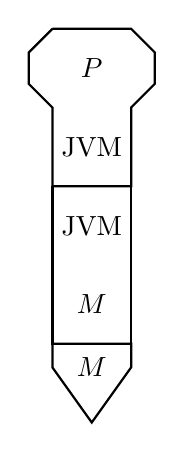
\begin{tikzpicture}
    \draw[thick] (0, 0) -- (1, 0) 
        -- (1.3, -0.3)
        -- (1.3, -0.7)
        -- (1, -1)
        -- (1, -2)
        -- (0, -2)
        -- (0, -1)
        -- (-0.3, -0.7)
        -- (-0.3, -0.3)
        -- (0, 0);
    \node at (0.5, -0.5) {$P$};
    \node at (0.5, -1.5) {JVM};
    
    \draw[thick] (1, -3) -- (1, -2)
        -- (1, -4) 
        -- (0, -4)
        -- (0, -2);
    \node at (0.5, -2.5) {JVM};
    \node at (0.5, -3.5) {$M$};
    
    \draw[thick] (0, 0-4) -- (1, 0-4)
        -- (1, -0.3-4)
        -- (0.5, -1-4)
        -- (0, -0.3-4)
        -- (0, 0-4);
    \node at (0.5, -0.3-4) {$M$};
    \end{tikzpicture}
\end{figure}
\noindent Here, the compilation stage is very slow, but it can be improved by bootstraping.

Assume that we have an $S \to T$ translator expressed in language $S$.
\begin{figure}[H]
    \centering
    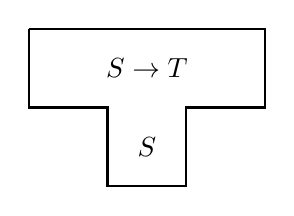
\begin{tikzpicture}
    \draw[thick] (0, 0) -- (3, 0)
        -- (3, -1)
        -- (2, -1)
        -- (2, -2)
        -- (1, -2)
        -- (1, -1)
        -- (0, -1)
        -- (0, 0);
    \node at (1.5, -0.5) {$S \to T$};
    \node at (1.5, -1.5) {$S$};
    \end{tikzpicture}
\end{figure}
\noindent We can use this translator to translate itself. This process is called bootstraping. It is a useful tool for improving an existing compiler. This is because it makes the compilation process faster, which makes it generate faster object code. We can bootstrap a portable compiler to make a true compiler, by translating virtual machine code into native machine code.

For example, consider the Java portable compiler kit.
\begin{figure}[H]
    \centering
    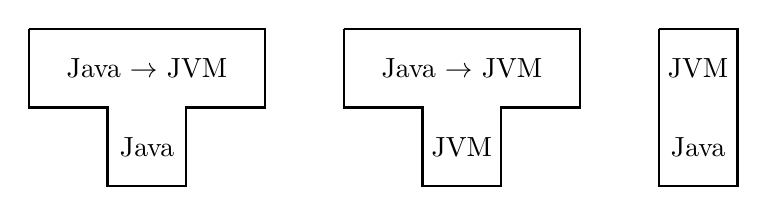
\begin{tikzpicture}
    \draw[thick] (0, 0) -- (3, 0)
        -- (3, -1)
        -- (2, -1)
        -- (2, -2)
        -- (1, -2)
        -- (1, -1)
        -- (0, -1)
        -- (0, 0);
    \node at (1.5, -0.5) {Java $\to$ JVM};
    \node at (1.5, -1.5) {Java};
    
    \draw[thick] (0+4, 0) -- (3+4, 0)
        -- (3+4, -1)
        -- (2+4, -1)
        -- (2+4, -2)
        -- (1+4, -2)
        -- (1+4, -1)
        -- (0+4, -1)
        -- (0+4, 0);
    \node at (1.5+4, -0.5) {Java $\to$ JVM};
    \node at (1.5+4, -1.5) {JVM};

    \draw[thick] (0+8, 0) -- (1+8, 0)
        -- (1+8, -2)
        -- (0+8, -2)
        -- (0+8, 0);
    \node at (0.5+8, -0.5) {JVM};
    \node at (0.5+8, -1.5) {Java};
    \end{tikzpicture}
\end{figure}
\noindent We also constructed a JVM interpreter in machine language $M$.
\begin{figure}[H]
    \centering
    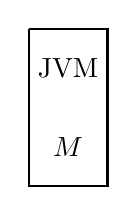
\begin{tikzpicture}
    \draw[thick] (0+8, 0) -- (1+8, 0)
        -- (1+8, -2)
        -- (0+8, -2)
        -- (0+8, 0);
    \node at (0.5+8, -0.5) {JVM};
    \node at (0.5+8, -1.5) {$M$};
    \end{tikzpicture}
\end{figure}
\noindent We can write a JVM $\to$ M translator in Java itself. We then compile it into JVM using the existing, slow compiler.
\begin{figure}[H]
    \centering
    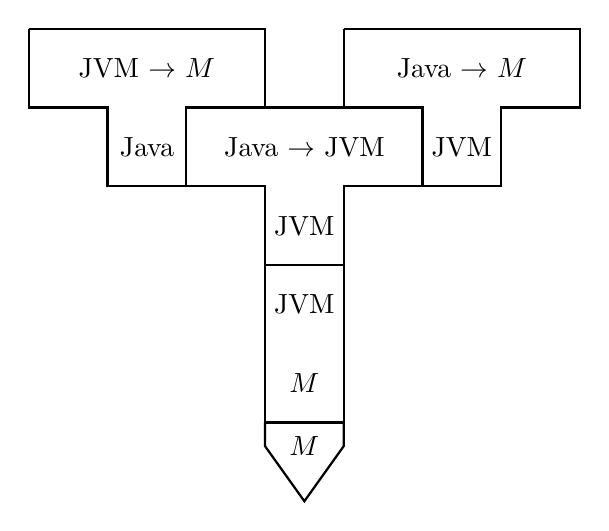
\begin{tikzpicture}
    \draw[thick] (0-1, 0) -- (3-1, 0)
        -- (3-1, -1)
        -- (2-1, -1)
        -- (2-1, -2)
        -- (1-1, -2)
        -- (1-1, -1)
        -- (0-1, -1)
        -- (0-1, 0);
    \node at (1.5-1, -0.5) {JVM $\to$ $M$};
    \node at (1.5-1, -1.5) {Java};
        
      \draw[thick] (0+1, 0-1) -- (3+1, 0-1)
        -- (3+1, -1-1)
        -- (2+1, -1-1)
        -- (2+1, -2-1)
        -- (1+1, -2-1)
        -- (1+1, -1-1)
        -- (0+1, -1-1)
        -- (0+1, 0-1);
    \node at (1.5+1, -0.5-1) {Java $\to$ JVM};
    \node at (1.5+1, -1.5-1) {JVM};

    \draw[thick] (0+3, 0) -- (3+3, 0)
        -- (3+3, -1)
        -- (2+3, -1)
        -- (2+3, -2)
        -- (1+3, -2)
        -- (1+3, -1)
        -- (0+3, -1)
        -- (0+3, 0);
    \node at (1.5+3, -0.5) {Java $\to$ $M$};
    \node at (1.5+3, -1.5) {JVM};

    \draw[thick] (1+2, -3-1) -- (1+2, -2-1)
        -- (1+2, -4-1) 
        -- (0+2, -4-1)
        -- (0+2, -2-1);
    \node at (0.5+2, -2.5-1) {JVM};
    \node at (0.5+2, -3.5-1) {$M$};

    \draw[thick] (0+2, 0-5) -- (1+2, 0-5)
        -- (1+2, -0.3-5)
        -- (0.5+2, -1-5)
        -- (0+2, -0.3-5)
        -- (0+2, 0-5);
    \node at (0.5+2, -0.3-5) {$M$};
    \end{tikzpicture}
\end{figure}
\noindent Next, we can use this JVM $\to$ M translator to translate itself.
\begin{figure}[H]
    \centering
    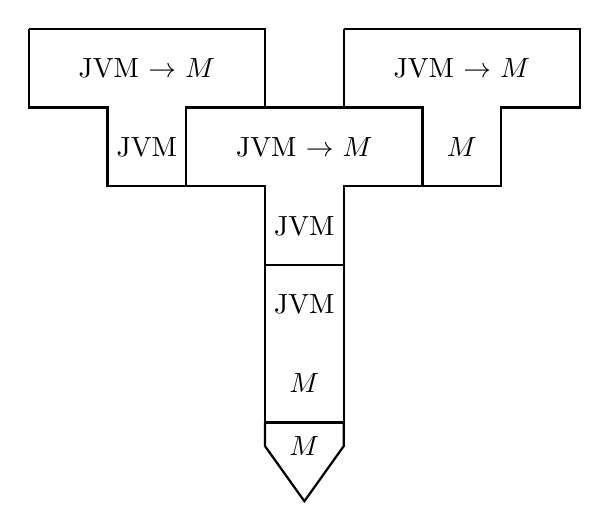
\begin{tikzpicture}
    \draw[thick] (0-1, 0) -- (3-1, 0)
        -- (3-1, -1)
        -- (2-1, -1)
        -- (2-1, -2)
        -- (1-1, -2)
        -- (1-1, -1)
        -- (0-1, -1)
        -- (0-1, 0);
    \node at (1.5-1, -0.5) {JVM $\to$ $M$};
    \node at (1.5-1, -1.5) {JVM};
        
      \draw[thick] (0+1, 0-1) -- (3+1, 0-1)
        -- (3+1, -1-1)
        -- (2+1, -1-1)
        -- (2+1, -2-1)
        -- (1+1, -2-1)
        -- (1+1, -1-1)
        -- (0+1, -1-1)
        -- (0+1, 0-1);
    \node at (1.5+1, -0.5-1) {JVM $\to$ $M$};
    \node at (1.5+1, -1.5-1) {JVM};

    \draw[thick] (0+3, 0) -- (3+3, 0)
        -- (3+3, -1)
        -- (2+3, -1)
        -- (2+3, -2)
        -- (1+3, -2)
        -- (1+3, -1)
        -- (0+3, -1)
        -- (0+3, 0);
    \node at (1.5+3, -0.5) {JVM $\to$ $M$};
    \node at (1.5+3, -1.5) {$M$};

    \draw[thick] (1+2, -3-1) -- (1+2, -2-1)
        -- (1+2, -4-1) 
        -- (0+2, -4-1)
        -- (0+2, -2-1);
    \node at (0.5+2, -2.5-1) {JVM};
    \node at (0.5+2, -3.5-1) {$M$};

    \draw[thick] (0+2, 0-5) -- (1+2, 0-5)
        -- (1+2, -0.3-5)
        -- (0.5+2, -1-5)
        -- (0+2, -0.3-5)
        -- (0+2, 0-5);
    \node at (0.5+2, -0.3-5) {$M$};
    \end{tikzpicture}
\end{figure}
\noindent This is the actual bootstrap. It generates the JVM $\to$ $M$ translator, expressed in $M$ machine code. Finally, we can translate the Java $\to$ JVM compiler into $M$ machine code.
\begin{figure}[H]
    \centering
    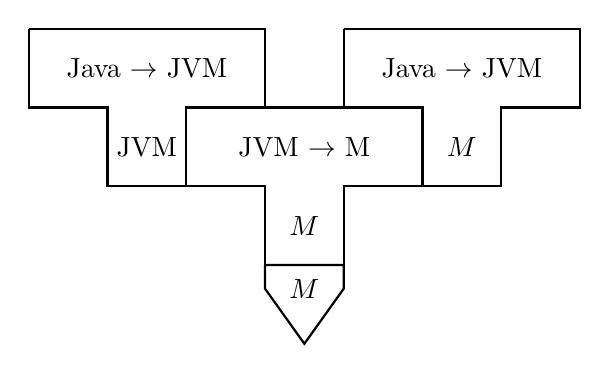
\begin{tikzpicture}
    \draw[thick] (0-1, 0) -- (3-1, 0)
        -- (3-1, -1)
        -- (2-1, -1)
        -- (2-1, -2)
        -- (1-1, -2)
        -- (1-1, -1)
        -- (0-1, -1)
        -- (0-1, 0);
    \node at (1.5-1, -0.5) {Java $\to$ JVM};
    \node at (1.5-1, -1.5) {JVM};
        
      \draw[thick] (0+1, 0-1) -- (3+1, 0-1)
        -- (3+1, -1-1)
        -- (2+1, -1-1)
        -- (2+1, -2-1)
        -- (1+1, -2-1)
        -- (1+1, -1-1)
        -- (0+1, -1-1)
        -- (0+1, 0-1);
    \node at (1.5+1, -0.5-1) {JVM $\to$ M};
    \node at (1.5+1, -1.5-1) {$M$};

    \draw[thick] (0+3, 0) -- (3+3, 0)
        -- (3+3, -1)
        -- (2+3, -1)
        -- (2+3, -2)
        -- (1+3, -2)
        -- (1+3, -1)
        -- (0+3, -1)
        -- (0+3, 0);
    \node at (1.5+3, -0.5) {Java $\to$ JVM};
    \node at (1.5+3, -1.5) {$M$};

    \draw[thick] (0+2, 0-3) -- (1+2, 0-3)
        -- (1+2, -0.3-3)
        -- (0.5+2, -1-3)
        -- (0+2, -0.3-3)
        -- (0+2, 0-3);
    \node at (0.5+2, -0.3-3) {$M$};
    \end{tikzpicture}
\end{figure}

Now, we have a 2-stage Java $\to$ $M$ compiler.
\begin{figure}[H]
    \centering
    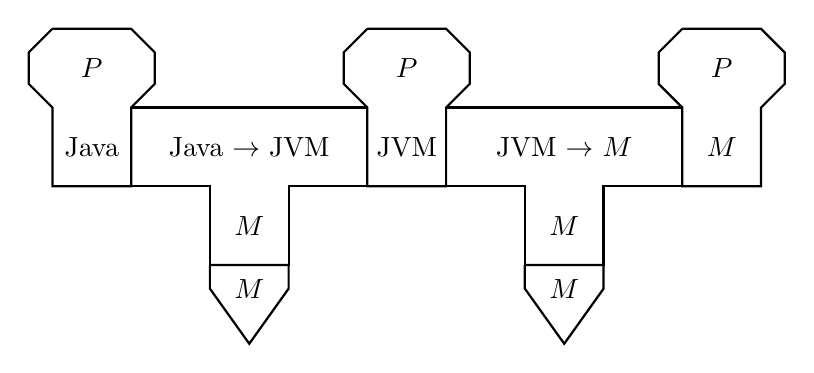
\begin{tikzpicture}
    \draw[thick] (0, 0) -- (1, 0) 
        -- (1.3, -0.3)
        -- (1.3, -0.7)
        -- (1, -1)
        -- (1, -2)
        -- (0, -2)
        -- (0, -1)
        -- (-0.3, -0.7)
        -- (-0.3, -0.3)
        -- (0, 0);
        \node at (0.5, -0.5) {$P$};
        \node at (0.5, -1.5) {Java};
        
      \draw[thick] (0+1, 0-1) -- (3+1, 0-1)
        -- (3+1, -1-1)
        -- (2+1, -1-1)
        -- (2+1, -2-1)
        -- (1+1, -2-1)
        -- (1+1, -1-1)
        -- (0+1, -1-1)
        -- (0+1, 0-1);
    \node at (1.5+1, -0.5-1) {Java $\to$ JVM};
    \node at (1.5+1, -1.5-1) {$M$};

    \draw[thick] (0+4, 0) -- (1+4, 0) 
        -- (1.3+4, -0.3)
        -- (1.3+4, -0.7)
        -- (1+4, -1)
        -- (1+4, -2)
        -- (0+4, -2)
        -- (0+4, -1)
        -- (-0.3+4, -0.7)
        -- (-0.3+4, -0.3)
        -- (0+4, 0);
        \node at (0.5+4, -0.5) {$P$};
        \node at (0.5+4, -1.5) {JVM};

    \draw[thick] (0+2, 0-3) -- (1+2, 0-3)
        -- (1+2, -0.3-3)
        -- (0.5+2, -1-3)
        -- (0+2, -0.3-3)
        -- (0+2, 0-3);
    \node at (0.5+2, -0.3-3) {$M$};
        
     \draw[thick] (0+5, 0-1) -- (3+5, 0-1)
        -- (3+5, -1-1)
        -- (2+5, -1-1)
        -- (2+5, -2-1)
        -- (1+5, -2-1)
        -- (1+5, -1-1)
        -- (0+5, -1-1)
        -- (0+5, 0-1);
    \node at (1.5+5, -0.5-1) {JVM $\to$ $M$};
    \node at (1.5+5, -1.5-1) {$M$};

    \draw[thick] (0+8, 0) -- (1+8, 0) 
        -- (1.3+8, -0.3)
        -- (1.3+8, -0.7)
        -- (1+8, -1)
        -- (1+8, -2)
        -- (0+8, -2)
        -- (0+8, -1)
        -- (-0.3+8, -0.7)
        -- (-0.3+8, -0.3)
        -- (0+8, 0);
        \node at (0.5+8, -0.5) {$P$};
        \node at (0.5+8, -1.5) {$M$};

    \draw[thick] (0+6, 0-3) -- (1+6, 0-3)
        -- (1+6, -0.3-3)
        -- (0.5+6, -1-3)
        -- (0+6, -0.3-3)
        -- (0+6, 0-3);
    \node at (0.5+6, -0.3-3) {$M$};
    \end{tikzpicture}
\end{figure}
\noindent This Java compiler is improved in two respects. It compilers faster since it is expressed in native machine code. It also generates faster object code.

\newpage

\section{Interpretation}
An $S$ interpreter accepts code expressed in language $S$ and immediately executes that code. Assuming that the code to be interpreted is just a sequence of simple instructions (with conditional and unconditional jumps), the interpreter:
\begin{itemize}
    \item first initialises the state,
    \item then repeatedly fetches, analyses and executes the next instruction, and
    \item updates the state as an instruction gets updated, as required.
\end{itemize}

Virtual machine code typically consists of:
\begin{itemize}
    \item load and store instructions,
    \item arithmetic and logical instructions,
    \item conditional and unconditional jumps, 
    \item call and return instructions, etc.
\end{itemize}
The virtual machine state typically consists of storage (code and data) along with registers (status, program counter, stack pointer, etc.).

\subsection{SVM}
Simple Virtual Machine (SVM) is suitable for executing programs in simple imperative PLs. Consider we have the following source code in a C-style language:
\begin{lstlisting}[language=java]
p = 1;
while (p < n) {
    p = 10 * p;
}
\end{lstlisting}
The corresponding SVM code for it is the following:
\begin{lstlisting}[language=SVM]
// load constant 1
LOADC 1
// store the constant 1 at address 2 (variable p)
STOREG 2
// load from address 2 (variable p)
LOADG 2
// load from address 1 (variable n)
LOADG 1
// compare p < n
COMPLT
// if false, jump to 29 = line 24 (and halt)
JUMPF 29
// load constant 10
LOADC 10
// load from address 2 (variable p)
LOADG 2
// multiply p and 10
MUL
// store p*10 to address 2
STOREG 2
// jump to 6 = line 6
JUMP 6
// halt
HALT
\end{lstlisting}

The SVM storage is composed of the code store and the data store. The code store is a fixed array of bytes (32 768 bytes) providing space for instructions. The data store is a fixed array of words (32 768 words) providing a stack to contain global and local data. The main registers for SVM are:
\begin{itemize}
    \item \texttt{pc} (program counter) points to the next instruction to be executed
    \item \texttt{sp} (stack pointer) points to the top of the stack
    \item \texttt{fp} (frame pointer) points to the base of the topmost frame
    \item \texttt{status} indicates whether the program is running, failed or halted.
\end{itemize}

The following image illustrates the code store of the SVM code above.
\begin{figure}[H]
    \centering
    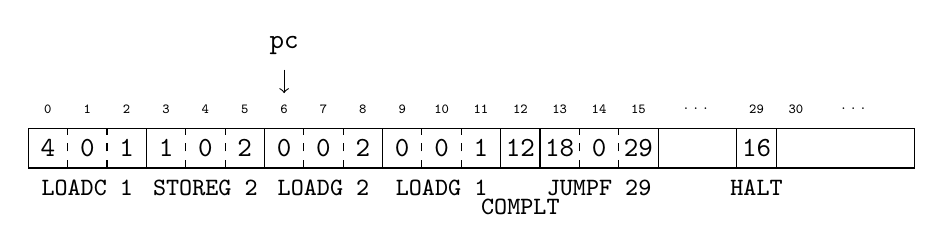
\begin{tikzpicture}
    \node at (0, 1) {\tiny\texttt{0}};
    \node at (0, 0.5) {\texttt{4}};
    \foreach \x[count=\i] in {0, 1, 1, 0, 2, 0, 0, 2, 0, 0, 1, 12, 18, 0, 29} {
        \node at (\i*0.5, 1) {\tiny\texttt{\i}};
        \node at (\i*0.5, 0.5) {\texttt{\x}};
    }
    \draw (-0.25, 0.25) -- (-0.25, 0.75) -- (11, 0.75) -- (11, 0.25) -- cycle;
    \foreach \i in {1, 2, 4, 5, 7, 8, 10, 11, 14, 15} {
        \draw[dashed] (\i*0.5-0.25, 0.25) -- (\i*0.5-0.25, 0.75);
    }
     \foreach \i in {3, 6, 9, 12, 13, 16, 18, 19} {
        \draw (\i*0.5-0.25, 0.25) -- (\i*0.5-0.25, 0.75);
    }
    \node at (8.25, 1) {\tiny$\dots$};
    
    \node at (9, 1) {\tiny\texttt{29}};
    \node at (9, 0.5) {\texttt{16}};

    \node at (9.5, 1) {\tiny\texttt{30}};
    \node at (10.25, 1) {\tiny$\dots$};
    
    \foreach \x[count=\i] in {LOADC 1, STOREG 2, LOADG 2, LOADG 1} {
        \node at (\i*1.5-1, 0) {\small\texttt{\x}};
    }
    \node at (6, -.25) {\small\texttt{COMPLT}};
    \node at (7, 0) {\small\texttt{JUMPF 29}};
    
    \node at (9, 0) {\small\texttt{HALT}};
    
    \draw[->] (3, 1.5) -- (3, 1.2);
    \node at (3, 1.8) {\texttt{pc}};
    
    \end{tikzpicture}
    \caption{An illustration of the code source.}
\end{figure}
\noindent Each instruction occupies 1, 2 or 3 bytes, e.g. \texttt{STOREG 2} occupies 3 bytes, while \texttt{COMPLT} occupies only 1. The register \texttt{pc} is pointing to 6, meaning that is the next instruction to be executed. The final part (after \texttt{30}) is the unused part of the code source.

Next, the following figure illustrates the data store.
\begin{figure}[H]
    \centering
    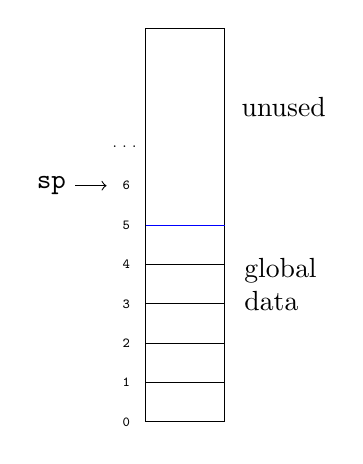
\begin{tikzpicture}
    \draw (0, 0) -- (1, 0)
        -- (1, 5)
        -- (0, 5)
        -- cycle;
    
    \foreach \i in {0, 1, ..., 5} {
        \node at (-0.25, \i*0.5) {\tiny\texttt{\i}};
        \draw (0, \i*0.5) -- (1, \i*0.5);
    }
    \node at (-0.25, 3) {\tiny\texttt{6}};
    \node at (-0.25, 3.5) {\tiny$\dots$};
    
    
    \node at (1.75, 4) {unused};
    \node[text width=1cm] at (1.75, 1.75) {global data};
    
    \draw[blue] (0, 2.5) -- (1, 2.5);
    
    \draw[->] (-.9, 3) -- (-.5, 3);
    \node at (-1.2, 3) {\texttt{sp}};
    \end{tikzpicture}
    \caption{An illustration of the data store at the start.}
\end{figure}
\noindent The register \texttt{sp} is pointing to 6, meaning that all the positions above 6 (including it) is unused and empty. At the bottom, there is only global data on the stack. As the program executes, we load further data, so we might end up at the following state.
\begin{figure}[H]
    \centering
    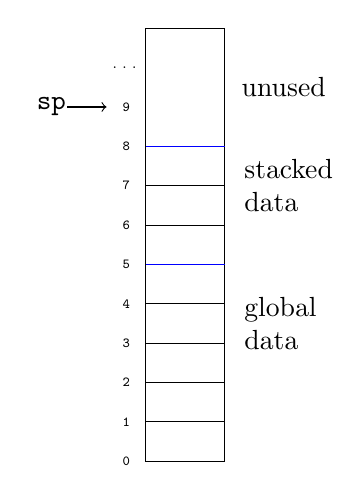
\begin{tikzpicture}
    \draw (0, 0) -- (1, 0)
        -- (1, 5.5)
        -- (0, 5.5)
        -- cycle;
    
    \foreach \i in {0, 1, ..., 8} {
        \node at (-0.25, \i*0.5) {\tiny\texttt{\i}};
        \draw (0, \i*0.5) -- (1, \i*0.5);
    }
    \draw[blue] (0, 2.5) -- (1, 2.5);
    \draw[blue] (0, 4) -- (1, 4);
    
    \node at (-0.25, 4.5) {\tiny\texttt{9}};
    \node at (-0.25, 5) {\tiny$\dots$};
    
    \node[text width=1cm] at (1.75, 3.5) {stacked data};
    \node[text width=1cm] at (1.75, 1.75) {global data};
    \node at (1.75, 4.75) {unused};
    
    \draw[->] (-1, 4.5) -- (-.5, 4.5);
    \node at (-1.2, 4.5) {\texttt{sp}};
    \end{tikzpicture}
    \caption{An illustration of the data store during execution.}
\end{figure}

The following is a simplified version of the SVM instruction set.
\begin{table}[H]
    \centering
    \begin{tabular}{|c|c|c|}
        \hline
        Opcode & Mnemonic & Behavior \\
        \hline
        6 & \texttt{ADD} & pop $w_2$; pop $w_1$; push $(w_1 + w_2)$ \\
        7 & \texttt{SUB} & pop $w_2$; pop $w_1$; push $(w_1 - w_2)$ \\
        8 & \texttt{MUL} & pop $w_2$; pop $w_1$; push $(w_1 * w_2)$ \\
        9 & \texttt{DOV} & pop $w_2$; pop $w_1$; push $(w_1 / w_2)$ \\
        10 & \texttt{CMPEQ} & pop $w_2$; pop $w_1$; push (if $w_1 = w_2$ then 1 else 0) \\
        11 & \texttt{CMPLT} & pop $w_2$; pop $w_1$; push (if $w_1 < w_2$ then 1 else 0) \\
        14 & \texttt{INV} & pop $w$; push (if $w=0$ then 1 else 0) \\
        0 & \texttt{LOADG} $d$ & $w$ $\leftarrow$ word at address $d$; push $w$ \\
        1 & \texttt{STOREG} $d$ & pop $w$; word at address $d$ $\leftarrow$ $w$ \\
        4 & \texttt{LOADC} $v$ & push $v$ \\
        16 & \texttt{HALT}  & status $\leftarrow$ halted \\
        17 & \texttt{JUMP} $c$ & pc $\leftarrow$ c \\
        18 & \texttt{JUMPF} $c$ & pop w; if $w = 0$ then pc $\leftarrow$ c \\
        19 & \texttt{JUMPT} $c$ & pop w; if $w \neq 0$ then pc $\leftarrow$ c \\
        \hline
    \end{tabular}
    \caption{The SVM Instruction Set}
\end{table}

We will illustrate how the data store changes as we execute the program. So, consider we are evaluating the following expression: \texttt{(7 + 3)*(5 - 2)}. In SVM, it is the following:
\begin{lstlisting}[language=SVM]
// load constant 7
LOADC 7
// load constant 3
LOADC 3
// add 7 and 3 = 10
ADD
// load constant 3
LOADC 5
// load constant 2
LOADC 2
// subtract 2 from 5 = 3
SUB
// multiply 10 and 3 = 30
MUL
\end{lstlisting}
We will illustrate the execution with the data store. Assume that the initial state of the stack is the following.
\begin{figure}[H]
    \centering
    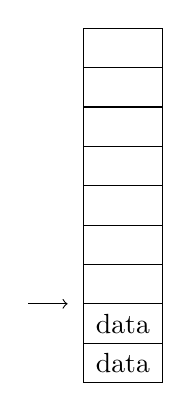
\begin{tikzpicture}
    \draw (0, 0) -- (1, 0)
        -- (1, 4.5)
        -- (0, 4.5)
        -- cycle;
    
    \foreach \i in {0, 1, ..., 8} {
        \draw (0, \i*0.5) -- (1, \i*0.5);
    }
    
    \foreach \x[count=\i] in {data, data} {
        \node at (0.5, 0.5*\i-0.25) {\x};
    }
    
    \draw[->] (-.7, 1) -- (-.2, 1);
    \end{tikzpicture}
\end{figure}
\noindent The arrow denotes the stack pointer \texttt{sp}. We first execute \texttt{LOADC 7}, which will add 7 to the stack.
\begin{figure}[H]
    \centering
    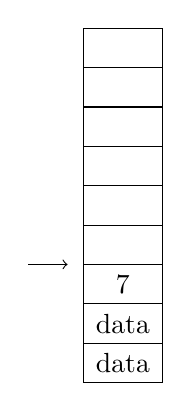
\begin{tikzpicture}
    \draw (0, 0) -- (1, 0)
        -- (1, 4.5)
        -- (0, 4.5)
        -- cycle;
    
    \foreach \i in {0, 1, ..., 8} {
        \draw (0, \i*0.5) -- (1, \i*0.5);
    }
    
    \foreach \x[count=\i] in {data, data, 7} {
        \node at (0.5, 0.5*\i-0.25) {\x};
    }
    
    \draw[->] (-.7, 1.5) -- (-.2, 1.5);
    \end{tikzpicture}
\end{figure}
\noindent Next, we execute \texttt{LOADC 3}, which will add 3 to the stack.
\begin{figure}[H]
    \centering
    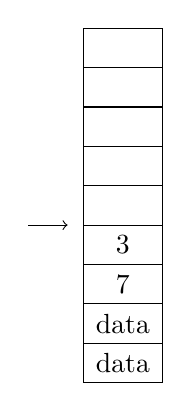
\begin{tikzpicture}
    \draw (0, 0) -- (1, 0)
        -- (1, 4.5)
        -- (0, 4.5)
        -- cycle;
    
    \foreach \i in {0, 1, ..., 8} {
        \draw (0, \i*0.5) -- (1, \i*0.5);
    }
    
    \foreach \x[count=\i] in {data, data, 7, 3} {
        \node at (0.5, 0.5*\i-0.25) {\x};
    }
    
    \draw[->] (-.7, 2) -- (-.2, 2);
    \end{tikzpicture}
\end{figure}
\noindent The next command is \texttt{ADD}. By its specification, we pop $w_2 = 3$ and $w_1 = 7$, and push $w_1 + w_2 = 10$.
\begin{figure}[H]
    \centering
    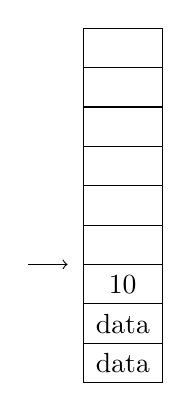
\begin{tikzpicture}
    \draw (0, 0) -- (1, 0)
        -- (1, 4.5)
        -- (0, 4.5)
        -- cycle;
    
    \foreach \i in {0, 1, ..., 8} {
        \draw (0, \i*0.5) -- (1, \i*0.5);
    }
    
    \foreach \x[count=\i] in {data, data, 10} {
        \node at (0.5, 0.5*\i-0.25) {\x};
    }
    
    \draw[->] (-.7, 1.5) -- (-.2, 1.5);
    \end{tikzpicture}
\end{figure}
\noindent The next command is \texttt{LOADC 5}. So, we push 5 to the stack.
\begin{figure}[H]
    \centering
    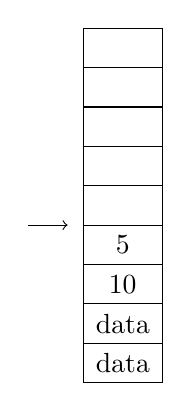
\begin{tikzpicture}
    \draw (0, 0) -- (1, 0)
        -- (1, 4.5)
        -- (0, 4.5)
        -- cycle;
    
    \foreach \i in {0, 1, ..., 8} {
        \draw (0, \i*0.5) -- (1, \i*0.5);
    }
    
    \foreach \x[count=\i] in {data, data, 10, 5} {
        \node at (0.5, 0.5*\i-0.25) {\x};
    }
    
    \draw[->] (-.7, 2) -- (-.2, 2);
    \end{tikzpicture}
\end{figure}
\noindent Now, we perform \texttt{LOADC 2}, when we push 2 to the stack.
\begin{figure}[H]
    \centering
    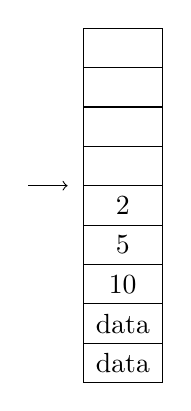
\begin{tikzpicture}
    \draw (0, 0) -- (1, 0)
        -- (1, 4.5)
        -- (0, 4.5)
        -- cycle;
    
    \foreach \i in {0, 1, ..., 8} {
        \draw (0, \i*0.5) -- (1, \i*0.5);
    }
    
    \foreach \x[count=\i] in {data, data, 10, 5, 2} {
        \node at (0.5, 0.5*\i-0.25) {\x};
    }
    
    \draw[->] (-.7, 2.5) -- (-.2, 2.5);
    \end{tikzpicture}
\end{figure}
\noindent The next command is \texttt{SUB}. So, we pop $w_2 = 2$ and $w_1 = 5$, and push $w_1 - w_2 = 3$.
\begin{figure}[H]
    \centering
    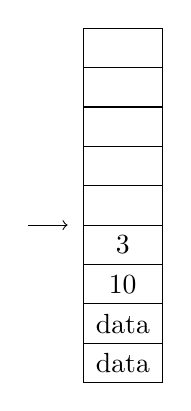
\begin{tikzpicture}
    \draw (0, 0) -- (1, 0)
        -- (1, 4.5)
        -- (0, 4.5)
        -- cycle;
    
    \foreach \i in {0, 1, ..., 8} {
        \draw (0, \i*0.5) -- (1, \i*0.5);
    }
    
    \foreach \x[count=\i] in {data, data, 10, 3} {
        \node at (0.5, 0.5*\i-0.25) {\x};
    }
    
    \draw[->] (-.7, 2) -- (-.2, 2);
    \end{tikzpicture}
\end{figure}
\noindent The final command is \texttt{MUL}. So, we pop $w_2 = 3$ and $w_1 = 10$, and push $w_1 * w_2 = 30$.
\begin{figure}[H]
    \centering
    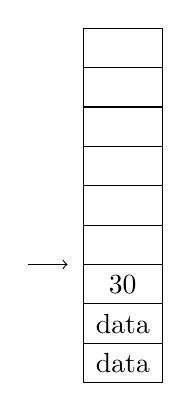
\begin{tikzpicture}
    \draw (0, 0) -- (1, 0)
        -- (1, 4.5)
        -- (0, 4.5)
        -- cycle;
    
    \foreach \i in {0, 1, ..., 8} {
        \draw (0, \i*0.5) -- (1, \i*0.5);
    }
    
    \foreach \x[count=\i] in {data, data, 30} {
        \node at (0.5, 0.5*\i-0.25) {\x};
    }
    
    \draw[->] (-.7, 1.5) -- (-.2, 1.5);
    \end{tikzpicture}
\end{figure}

\subsection{Writing interpreters}
Interpreters are commonly written in C or Java. In such an interpreter, the virtual machine state is represented by a group of variables. Each instruction is executed by inspecting and/or updating the virtual machine state.

For the SVM interpreter in a Java, the following is the representation of the instructions.
\begin{lstlisting}[language=java]
final byte
    LOADG = 0, STOREG = 1,
    LOADL = 2, STOREL = 3,
    LOADC = 4,
    ADD = 6, SUB = 7,
    MUL = 8, DIV = 9,
    CMPEQ = 10,
    CMPLT = 12, CMPGT = 13,
    INV = 14, INC = 14,
    HALT = 16, JUMP = 17,
    JUMPF = 18, JUMPT = 19,
\end{lstlisting}
Each instruction is a byte, and given a value, e.g. \texttt{ADD} is 6, and so on. The virtual machine state is given by the following.
\begin{lstlisting}[language=java]
byte[] code; // code store
int[] data; // data store
int pc, cl, sp, fp, status; // registers
final byte
    RUNNING = 0,
    FAILED = 1,
    HALTED = 2;
\end{lstlisting}
The interpreter initialises the state, then repeatedly fetches and executes the instructions. The interpret method is outlined below:
\begin{lstlisting}[language=java]
void interpret () {
    // Initialise the state
    status = RUNNING;
    sp = 0; fp = 0; pc = 0;
    do {
        // Fetch the next instruction
        byte opcode = code[pc++];
        // Execute this instruction
        ...
    } while (status == RUNNING);
}
\end{lstlisting}
To execute an instruction, we first inspect its opcode, which is given below.
\begin{lstlisting}[language=java]
// Execute this instruction:
switch (opcode) {
    case LOADG: ...
    case STOREG: ...
    ...
    case ADD: ...
    case CMPLT: ...
    ...
    case HALT: ...
    case JUMP: ...
    case JUMPT: ...
    ...
}
\end{lstlisting}
Within each case, we have the instructions to execute it, e.g. \texttt{ADD} and \texttt{CMPLT} are given below.
\begin{lstlisting}[language=java]
case ADD: {
    int w2 = data[--sp];
    int w1 = data[--sp];
    data[sp++] = w1 + w2;
    break; 
}
case CMPLT: {
    int w2 = data[--sp];
    int w1 = data[--sp];
    data[sp++] = w1 < w2 ? 1 : 0;
    break; 
}
\end{lstlisting}
The load and store instructions are given below.
\begin{lstlisting}[language=java]
case LOADG: {
    // gives the address d for the data store (2-byte operand)
    int d = code[pc++] << 8 | code[pc++];
    data[sp++] = data[d];
    break; 
}
case STOREG: {
    int d = code[pc++] << 8 | code[pc++];
    data[d] = data[--sp];
    break; 
}
\end{lstlisting}
The following are halting and jumping instructions.
\begin{lstlisting}[language=java]
case HALT: {
    status = HALTED;
    break; 
}
case JUMP: {
    // fetch 2-byte operand
    int c = ...;
    pc = c;
    break; 
}
case JUMPT: {
    // fetch 2-byte operand
    int c = ...;
    int w = data[--sp];
    if (w != 0) pc = c;
    break; 
}
\end{lstlisting}

\newpage

\section{Compilation}
An $S \to T$ compiler translates a source program in $S$ to object code in $T$ given that it conforms the source language's syntax and scope/type rules. This suggests that the compilation stage should be decomposed into three phases: syntactic analysis, contextual analysis and code generation. 

In syntactic analysis, we parse the source program to check whether it is well-formed, and to determine its phrase structure, in accordance with the source language's syntax. In contextual analysis, we analyse the parsed program to check whether it conforms the source language's scope and type rules. In code generation, we translate the parsed program to object code, in accordance with the source language's semantics.

The following figure illustrates data flow between the phases:
\begin{figure}[H]
    \centering
    \begin{tikzpicture}
        \node[draw, text width=2cm, align=center] (SA) at (0, 0) {syntactic analysis};
        \node[draw, text width=2cm, align=center] (CA) at (3.5, 0) {contextual analysis};
        \node[draw, text width=2cm, align=center] (CG) at (7, 0) {code \\ generation};
        
        \draw[->] (-2.5, 0) -- (SA);
        \node[text width=2cm, align=center] at (-1.75, -.5) {source program};
        \draw[->] (SA) -- (0, -2);
        \node[text width=2cm, align=center] at (0.75, -1.5) {syntactic errors};
        
        \draw[->] (SA) -- (CA);
        \node[text width=2cm, align=center] at (1.75, -.2) {AST};
        \draw[->] (CA) -- (3.5, -2);
        \node[text width=2cm, align=center] at (4.5, -1.5) {scope/type errors};
        
        \draw[->] (CA) -- (CG);
        \node[text width=2cm, align=center] at (5.25, -.2) {AST};
        \draw[->] (CG) -- (7, -2);
        \node[text width=2cm, align=center] at (7.75, -1.5) {object program};
    \end{tikzpicture}
    \caption{The data flow between the compilation phases.}
\end{figure}
\noindent Source program is given as input to the syntactic analysis phase. If there are no syntactic errors, we can transform it into an abstract syntax tree (AST). This is then analysed contextually. If there are no type or scope errors, then the AST will get annotated. This is then used to generate the object program. An AST is a convenient way to represent a source program after syntactic analysis.

\subsection{Fun}
Fun is a simple imperative language. A Fun program declares some global variables and some procedures/functions, always including a procedure named \texttt{main()}. A Fun procedure/function may have a single parameter. It may also declare local variables. A function returns a result, but a procedure does not. Fun has two data types- \texttt{bool} and \texttt{int}. Commands in Fun can be:
\begin{itemize}
    \item assignment,
    \item procedure/function call,
    \item if command,
    \item while command, and
    \item sequential command.
\end{itemize}

The following is a simple Fun program.
\begin{lstlisting}[language=fun]
# returns n!
func int fact (int n): 
    int f = 1
    while n > 1:
        f = f * n
        n = n - 1
    .
    return f 
.

proc main ():
    int num = read()
    write(num)
    write(fact(num)) 
.
\end{lstlisting}
Fun programs are free-format, i.e. spaces, tabs and EOLs are not significant. 

The following is an extract of the Fun grammar, in EBNF form:
\begin{align*}
    \textit{prog } =& \textit{ var-decl}^* \textit{ proc-decl}^+ \textit{ eof} \\
    \textit{var-decl } =& \textit{ type id } \text{`}\texttt{=}\text{'} \textit{ expr} \\
    \textit{type } =& \text{ `}\texttt{bool}\text{'} \\
    |\hspace{2pt} & \text{ `}\texttt{int}\text{'} \\
    \textit{com } =& \textit{ id } \text{`}\texttt{=}\text{'} \textit{ expr} \\
    |\hspace{2pt} & \texttt{ if } \textit{expr} \text{ `}\texttt{:}\text{'} \textit{ seq-com} \text{ `}\texttt{.}\text{'} \\
    |\hspace{2pt} & \ \dots \\
    \textit{seq-com } =& \textit{ com}^* \\
    \textit{expr } =& \textit{ sec-expr} \dots \\
    \textit{sec-expr } =& \textit{ prim-expr } ((\text{`}\texttt{+}\text{' } | \text{`}\texttt{-}\text{' } | \text{ `}\texttt{*}\text{' } | \text{ `}\texttt{/}\text{'}) \textit{prim-expr})^* \\
    \textit{prim-expr } =& \textit{ num} \\
    |\hspace{2pt} & \textit{ id} \\
    |\hspace{2pt} & \text{ `}\texttt{(}\text{ '} \textit{expr } \text{`}\texttt{)}\text{'} \\
    |\hspace{2pt} & \ \dots
\end{align*}

The Fun compiler generates SVM code. It is expressed in Java. The tombstone is given below.
\begin{figure}[H]
    \centering
    \begin{tikzpicture}
    \draw[thick] (0, 0) -- (3, 0)
        -- (3, -1)
        -- (2, -1)
        -- (2, -2)
        -- (1, -2)
        -- (1, -1)
        -- (0, -1)
        -- (0, 0);
    \node at (1.5, -0.5) {Fun $\to$ SVM};
    \node at (1.5, -1.5) {Java};
    \end{tikzpicture}
\end{figure}
\noindent The compiler contains the following classes:
\begin{itemize}
    \item syntactic analyser (\texttt{FunLexer}, \texttt{FunParser}),
    \item contextual analyser (\texttt{FunChecker}),
    \item code generator (\texttt{FunEncoder}).
\end{itemize}
The compiler calls each of these in turn:
\begin{itemize}
    \item The syntactic analyser lexes and parses the source program, printing any error messages and generates an AST. Then, the AST is printed.
    \item The contextual analyser performs scope and type checking, printing any error messages.
    \item The code generator emits object code into the SVM code store. Then, the object code is printed.
\end{itemize}
Compilation is terminated after syntactic or contextual analysis if any errors are detected.

The driver \texttt{FunRun} compiles the source program into an SVM object program. If no errors are detected, it calls the SVM interpreter to run the object program.

\subsection{AST}
An abstract syntax tree (AST) is a convenient way to represent a source program's phrase structure. The structure of an AST is the following:
\begin{itemize}
    \item Each leaf node represents an identifier or literal.
    \item Each internal node corresponds to a source language construct (e.g. a variable declaration or while-command). The internal node's subtrees represent the parts of that construct.
\end{itemize}
ASTs are much more compact than syntax trees.

For example, the AST for the expression \texttt{(x + 13) * (y - z)} in Fun is the following:
\begin{figure}[H]
    \centering
    \begin{tikzpicture}[
        level 1/.style={sibling distance=3cm},
        level 2/.style={sibling distance=1cm},
    ]
    \node[ellipse, draw] {Times}
    child {
        node[ellipse, draw] {Plus}
        child {
            node[label=-90:Id, draw] {\texttt{x}}
        }
        child {
            node[label=-90:Num, draw] {\texttt{3}}
        }
    }
    child {
        node[ellipse, draw] {Minus}
        child {
            node[label=-90:Id, draw] {\texttt{y}}
        }
        child {
            node[label=-90:Id, draw] {\texttt{z}}
        }
    };
    \end{tikzpicture}
\end{figure}
\noindent In the AST, we make no distinct between \textit{expr}, \textit{sec-expr}, etc. They are all treated as expressions. This is one of the ways an AST is compact.

Now, consider the following program in Fun:
\begin{lstlisting}[language=Fun]
if n > 0:
    n = n - 1
    write(n); .
\end{lstlisting}
The corresponding AST is the following:
\begin{figure}[H]
    \centering
    \begin{tikzpicture}[
        level 1/.style={sibling distance=5cm},
        level 2/.style={sibling distance=3.5cm},
        level 3/.style={sibling distance=1.5cm},
    ]
    \node[ellipse, draw] {IF}
    child[
        level 2/.style={sibling distance=1.5cm},
    ] {
        node[ellipse, draw] {GT}
        child {
            node[draw, label=-90:ID] {\texttt{n}}
        }
        child {
            node[draw, label=-90:NUM] {\texttt{0}}
        }
    }
    child {
        node[ellipse, draw] {SEQ}
        child {
            node[ellipse, draw] {ASSN}
            child {
                node[draw, label=-90:ID] {\texttt{n}}
            }
            child {
                node[ellipse, draw] {MINUS}
                child {
                    node[draw, label=-90:ID] {\texttt{n}}
                }
                child {
                    node[draw, label=-90:NUM] {\texttt{1}}
                }
            }
        }
        child {
            node[ellipse, draw] {PROCCALL}
            child {
                node[draw, label=-90:ID] {\texttt{write}}
            }
            child {
                node[draw, label=-90:ID] {\texttt{n}}
            }
        }
    };
    \end{tikzpicture}
\end{figure}

Now, we will look at all the Fun ASTs. For assignment, the AST is the following:
\begin{figure}[H]
    \centering
    \begin{tikzpicture}
        \node[ellipse, draw] {ASSN}
        child {
            node[draw, label=-90:ID, inner sep=2mm] {}
        }
        child {
            node[ellipse, draw] {expr}
        };
    \end{tikzpicture}
\end{figure}
\noindent The assignment is given by an identifier, which is given the value of some expression. The procedure call AST is the following:
\begin{figure}[H]
    \centering
    \begin{tikzpicture}
        \node[ellipse, draw] {PROCCALL}
        child {
            node[draw, label=-90:ID, inner sep=2mm] {}
        }
        child {
            node[ellipse, draw] {expr}
        };
    \end{tikzpicture}
\end{figure}
\noindent The expression is the same as assignment- we have an identifier for the procedure name, and its parameter is some expression. Next, the AST for a sequence of commands is the following:
\begin{figure}[H]
    \centering
    \begin{tikzpicture}
        \node[ellipse, draw] {SEQ}
        child {
            node[ellipse, draw] {com}
        }
        child {
            node {$\dots$}
        };
    \end{tikzpicture}
\end{figure}
\noindent It is composed of a sequence of commands, and we must have at least one command. Now, the if AST is given below:
\begin{figure}[H]
    \centering
    \begin{tikzpicture}
        \node[ellipse, draw] {IF}
        child {
            node[ellipse, draw] {expr}
        }
        child {
            node[ellipse, draw] {com}
        };
    \end{tikzpicture}
\end{figure}
\noindent We have an expression (that evaluates to true or false), and if it evaluates to true, we run the command. The AST for ifelse is given below:
\begin{figure}[H]
    \centering
    \begin{tikzpicture}
        \node[ellipse, draw] {IFELSE}
        child {
            node[ellipse, draw] {expr}
        }
        child {
            node[ellipse, draw] {com1}
        }
        child {
            node[ellipse, draw] {com2}
        };
    \end{tikzpicture}
\end{figure}
\noindent Here, we have an expression (that evaluates to true or false), and if it evaluates to true, we run the command com1, and otherwise, com2. The AST for a while loop is given below.
\begin{figure}[H]
    \centering
    \begin{tikzpicture}
        \node[ellipse, draw] {WHILE}
        child {
            node[ellipse, draw] {expr}
        }
        child {
            node[ellipse, draw] {com}
        };
    \end{tikzpicture}
\end{figure}
\noindent Here too, We have an expression (that evaluates to true or false), and if it evaluates to true, we run the command com1, and we rerun the expression and so on.

Now, we will look at ASTs for Fun expressions. There are 4 literal expressions, shown below.
\begin{figure}[H]
    \centering
    \begin{tikzpicture}
        \node[draw] at (0, 0) {\texttt{FALSE}};
        
        \node[draw] at (2, 0) {\texttt{TRUE}};
        
        \node[label=-90:NUM] at (4, 0) {};
        \draw (3.5, -.1) -- (4.5, -.1) -- (4.5, .2) -- (3.5, .2) -- cycle;
        
        \node[label=-90:ID] at (6, 0) {};
        \draw (5.5, -.1) -- (6.5, -.1) -- (6.5, .2) -- (5.5, .2) -- cycle;
    \end{tikzpicture}
\end{figure}
\noindent The literals are the boolean values \texttt{true} and \texttt{false}, numbers and identifiers. The AST for the function call expression is the following:
\begin{figure}[H]
    \centering
    \begin{tikzpicture}
        \node[ellipse, draw] {FUNCCALL}
        child {
            node[draw, label=-90:ID, inner sep=2mm] {}
        }
        child {
            node[ellipse, draw] {expr}
        };
    \end{tikzpicture}
\end{figure}
\noindent We have a name for the function, and the value of the parameter is some expression. Moreover, the arithmetic operations (plus, minus, times, div) are also expressions, with AST given below:
\begin{figure}[H]
    \centering
    \begin{tikzpicture}[
        level 1/.style={sibling distance=2.5cm}
    ]
        \node[ellipse, draw] at (0, 0) {PLUS}
        child {
            node[ellipse, draw] {expr1}
        }
        child {
            node[ellipse, draw] {expr2}
        };
        
        
        \node[ellipse, draw] at (4.5, 0) {MINUS}
        child {
            node[ellipse, draw] {expr1}
        }
        child {
            node[ellipse, draw] {expr2}
        };
        
        \node[ellipse, draw] at (0, -3) {MUL}
        child {
            node[ellipse, draw] {expr1}
        }
        child {
            node[ellipse, draw] {expr2}
        };
        
        
        \node[ellipse, draw] at (4.5, -3) {DIV}
        child {
            node[ellipse, draw] {expr1}
        }
        child {
            node[ellipse, draw] {expr2}
        };
    \end{tikzpicture}
\end{figure}
\noindent In each case, we have two expressions, and the operation is applied in the natural way. We also have comparison operations, whose AST is given below:
\begin{figure}[H]
    \centering
    \begin{tikzpicture}[
        level 1/.style={sibling distance=2.5cm}
    ]
        \node[ellipse, draw] at (0, 0) {EQ}
        child {
            node[ellipse, draw] {expr1}
        }
        child {
            node[ellipse, draw] {expr2}
        };
        
        
        \node[ellipse, draw] at (4.5, 0) {LT}
        child {
            node[ellipse, draw] {expr1}
        }
        child {
            node[ellipse, draw] {expr2}
        };
        
        \node[ellipse, draw] at (2.25, -3) {GT}
        child {
            node[ellipse, draw] {expr1}
        }
        child {
            node[ellipse, draw] {expr2}
        };
    \end{tikzpicture}
\end{figure}
\noindent We compare two expressions (for equality, less than or greater than). Next, the AST for the not expression is given below.
\begin{figure}[H]
    \centering
    \begin{tikzpicture}
        \node[ellipse, draw] at (4.5, -3) {NOT}
        child {
            node[ellipse, draw] {expr}
        };
    \end{tikzpicture}
\end{figure}
\noindent The expression evaluates to some boolean value, so the result will be the opposite boolean.

The AST for a Fun program is given below.
\begin{figure}[H]
    \centering
    \begin{tikzpicture}[
        level 1/.style={sibling distance=2.5cm}
    ]
        \node[ellipse, draw] {PROG}
        child {
            node[ellipse, draw] {var-decl}
        }
        child {
            node {$\dots$}
        }
        child {
            node[ellipse, draw] {prog-decl}
        }
        child {
            node {$\dots$}
        };
    \end{tikzpicture}
\end{figure}
\noindent So, a program is a sequence of variable declarations and a sequence of program declarations. The AST for variable declarations is given below.
\begin{figure}[H]
    \centering
    \begin{tikzpicture}
        \node[ellipse, draw] {VAR}
        child {
            node[ellipse, draw] {type}
        }
        child {
            node[draw, label=-90:ID, inner sep=2mm] {}
        }
        child {
            node[ellipse, draw] {expr}
        };
    \end{tikzpicture}
\end{figure}
\noindent We specify the type of a variable, call it an identifier, and assign it the value of some expression. The ASTs for Fun types is given below:
\begin{figure}[H]
    \centering
    \begin{tikzpicture}
        \node[draw, label=-90:BOOL] at (0, 0) {\texttt{BOOL}};
        \node[draw, label=-90:INT] at (2, 0) {\texttt{INT}};
    \end{tikzpicture}
\end{figure}
\noindent In Fun, there are only 2 types- bool and int. The AST for a procedure declaration is given below.
\begin{figure}[H]
    \centering
    \begin{tikzpicture}[
        level 1/.style={sibling distance=2.5cm}
    ]
        \node[ellipse, draw] {PROC}
        child {
            node[draw, label=-90:ID, inner sep=2mm] {}
        }
        child {
            node[ellipse, draw] {noformal}
        }
        child {
            node[ellipse, draw] {var-decl}
        }
        child {
            node {$\dots$}
        }
        child {
            node[ellipse, draw] {com}
        };
    \end{tikzpicture}
\end{figure}
\noindent A procedure has an identifier, a noformal (parameter), followed by some variable declarations and command for the body. The AST for a function declaration is the following.
\begin{figure}[H]
    \centering
    \begin{tikzpicture}[
        level 1/.style={sibling distance=2cm},
        scale=0.8
    ]
        \node[ellipse, draw] {FUNC}
        child {
            node[draw, ellipse] {type}
        }
        child {
            node[draw, label=-90:ID, inner sep=2mm] {}
        }
        child {
            node[ellipse, draw] {formal}
        }
        child {
            node[ellipse, draw] {var-decl}
        }
        child {
            node {$\dots$}
        }
        child {
            node[ellipse, draw] {com}
        }
        child {
            node[ellipse, draw] {expr}
        };
    \end{tikzpicture}
\end{figure}
\noindent We have the return type, identifier, the parameter formal, command and expression. The AST for formal and nonformal parameters is given below.
\begin{figure}[H]
    \centering
    \begin{tikzpicture}
        \node[ellipse, draw] at (0, 0) {FORMAL}
        child {
            node[ellipse, draw] {type}
        }
        child {
            node[draw, label=-90:ID, inner sep=2mm] {}
        };
        
        \node[ellipse, draw] at (4, 0) {NOFORMAL};
    \end{tikzpicture}
\end{figure}
\noindent A formal parameter represents a single parameter (for functions) and no parameters (for procedures).

We will now create an AST from a program. So, consider the following program.
\begin{lstlisting}[language=fun]
int n = 15
# div program
proc main ():
    while n > 1:
        n = n/2 .
.
\end{lstlisting}
\noindent Then, its AST is the following, after syntactical analysis of the program.
\begin{figure}[H]
    \centering
    \begin{tikzpicture}[
        level 1/.style={sibling distance=5cm},
        level 2/.style={sibling distance=3cm},
        level 3/.style={sibling distance=2cm},
        level 4/.style={sibling distance=1cm},
    ]
        \node[ellipse, draw] {PROG}
        child[
            level 2/.style={sibling distance=1cm}
        ] {
            node[ellipse, draw] {VAR}
            child {
                node[draw, label=-90:INT] {\texttt{int}}
            }
            child {
                node[draw, label=-90:ID] {\texttt{n}}
            }
            child {
                node[draw, label=-90:NUM] {\texttt{15}}
            }
        }
        child {
            node[ellipse, draw] {PROC}
            child {
                node[draw, label=-90:ID] {\texttt{main}}
            }
            child {
                node[ellipse, draw] {NOFORMAL}
            }
            child {
                node[ellipse, draw] {WHILE}
                child {
                    node[ellipse, draw] {GT}
                    child {
                        node[draw, label=-90:ID] {\texttt{n}}
                    }
                    child {
                        node[draw, label=-90:NUM] {\texttt{1}}
                    }
                }
                child {
                    node[ellipse, draw] {ASSN}
                    child {
                        node[draw, label=-90:ID] {\texttt{n}}
                    }
                    child {
                        node[ellipse, draw] {DIV}
                        child {
                            node[draw, label=-90:ID] {\texttt{n}}
                        }
                        child {
                            node[draw, label=-90:NUM] {\texttt{2}}
                        }
                    }
                }
            }
        };
    \end{tikzpicture}
\end{figure}
\noindent During contextual analysis, we do a type check and a scope check. Within the program, we find that we have a global variable \texttt{n:INT} and a global procedure $\texttt{main:VOID}\to \texttt{VOID}$. This is stored in a type table, specifying the name and the type. Using this, we can check the type and infer the type of each expression. This is given in the annotated AST below.
\begin{figure}[H]
    \centering
    \begin{tikzpicture}[
        level 1/.style={sibling distance=5cm},
        level 2/.style={sibling distance=3cm},
        level 3/.style={sibling distance=2cm},
        level 4/.style={sibling distance=1cm},
    ]
        \node[ellipse, draw] {PROG}
        child[
            level 2/.style={sibling distance=1cm}
        ] {
            node[ellipse, draw] {VAR}
            child {
                node[draw, label=-90:INT] {\texttt{int}}
            }
            child {
                node[draw, label=-90:ID] {\texttt{n}}
            }
            child {
                node[draw, label=-90:NUM, fill=blue!50, opacity=0.5] {\texttt{15}}
            }
        }
        child {
            node[ellipse, draw] {PROC}
            child {
                node[draw, label=-90:ID] {\texttt{main}}
            }
            child {
                node[ellipse, draw] {NOFORMAL}
            }
            child {
                node[ellipse, draw] {WHILE}
                child {
                    node[ellipse, draw, fill=red!50, opacity=0.5] {GT}
                    child {
                        node[draw, label=-90:ID, fill=blue!50, opacity=0.5] {\texttt{n}}
                    }
                    child {
                        node[draw, label=-90:NUM, fill=blue!50, opacity=0.5] {\texttt{1}}
                    }
                }
                child {
                    node[ellipse, draw] {ASSN}
                    child {
                        node[draw, label=-90:ID, fill=blue!50, opacity=0.5] {\texttt{n}}
                    }
                    child {
                        node[ellipse, draw, fill=blue!50, opacity=0.5] {DIV}
                        child {
                            node[draw, label=-90:ID, fill=blue!50, opacity=0.5] {\texttt{n}}
                        }
                        child {
                            node[draw, label=-90:NUM, fill=blue!50, opacity=0.5] {\texttt{2}}
                        }
                    }
                }
            }
        };
    \end{tikzpicture}
\end{figure}
\noindent A red value represents a \texttt{BOOL}, while a blue value represents an \texttt{INT}. Finally, we can create the SVM object code.
\begin{lstlisting}[language=SVM]
// load constant 15
LOADC 15
// go to 7 = line 8
CALL 7
// stop
HALT
// load the variable at address 0 (variable n)
LOADG 0
// load constant 1
LOADC 1
// compare n > 1
COMPGT
// if false, go to 30 = line 26 (and halt)
JUMPF 30
// load the variable at address 0 (variable n)
LOADG 0
// load constant 2
LOADC 2
// compute n/2
DIV
// store the result at address 0
STOREG 0
// go to 7 = line 8
JUMP 7
// return the value at address 0 (variable n)
RETURN 0
\end{lstlisting}

\end{document}
